% ============================================================================
% 超越表示保真度：跨模型 KV 传输的功能兼容性（中文译本）
% 这是 paper/main.tex 的中文译本：内容、数字、图表与标签与英文稿一一对应。
% 图表：paper/figures/gen_paper_figures.py（figures4papers 风格）。
% 正文中的每一个经验数字都转录自「可复现性声明」中列出的项目结果摘要；
% 那些摘要中未保留的量，正文中如实说明为未保留；宏 \need{} 未使用。
% 编译：tools/tectonic/tectonic.exe -X compile main_zh.tex（xelatex 引擎）。
% ============================================================================
\documentclass[11pt]{article}

\usepackage[margin=1in]{geometry}
\usepackage[UTF8,scheme=chinese,fontset=windows]{ctex}
\usepackage{booktabs}
\usepackage{graphicx}
\usepackage{multirow}
\usepackage{amsmath}
\usepackage{amssymb}
\usepackage[colorlinks=true,linkcolor=blue,citecolor=blue,urlcolor=blue]{hyperref}

\newcommand{\dll}{\Delta\text{LL}}
\newcommand{\emscore}{\text{EM}}
\newcommand{\need}[1]{\textbf{[需要数据：#1]}}
\setlength{\emergencystretch}{2.5em}
\setlength{\tabcolsep}{4pt}

% --- PDF 元数据（与英文稿一致） ---------------------------------------------
\hypersetup{
  pdftitle={超越表示保真度：跨模型 KV 传输的功能兼容性},
  pdfauthor={Zhang Xuemin, Zhong Liheng, Hu Liangbin, Yu Junpeng, Yi Kun},
  pdfsubject={机器学习；自然语言处理；高效推理},
  pdfkeywords={KV 缓存传输, 跨模型推理, 功能兼容性, 表示保真度, 消费空间对齐, 评测方法学},
  bookmarksnumbered=true,
}

\title{超越表示保真度：\\
跨模型 KV 传输的功能兼容性}

\author{%
  Zhang Xuemin\thanks{\texttt{zxm0813@gmail.com}}
  \and Zhong Liheng\thanks{\texttt{lihengzhong@berkeley.edu}}
  \and Hu Liangbin\thanks{\texttt{huliangbing2000@163.com}}
  \and Yu Junpeng\thanks{\texttt{yjp603@163.com}}
  \and Yi Kun\thanks{\texttt{yikun@bit.edu.cn}}%
}
\date{}

\begin{document}
\maketitle

\begin{center}
\small 本文为同名英文稿（\texttt{paper/main.tex}）的中文译本，数字、表格、图与标签与英文稿一一对应。
\end{center}

% ============================================================================
\begin{abstract}
在语言模型之间传输键--值（KV）缓存，有望在模型升级或组装集成模型时免去重新计算。
我们在 Qwen3 家族内部（$0.6$B--$8$B；六个教师--学生模型对；三个随机种子）重新审视
这一主张，给出一个诊断性的负结果以及随之而来的建设性修复方案。

本工作早期版本所用的评测协议高估了迁移。它的贪心精确匹配（EM）指标是在一个已经
推进过提问与标准答案的缓存上计算的，并且把最后一个提问 token 重新作为生成的第一个
输入；这两个缺陷都在该实现中，我们用全前缀（full-prefill）参考实现在完整的 Self 测试
集上校验了修正后的评测器（归一化 EM 一致率 $0.929$--$0.982$；首 token top-1 一致率
$0.929$--$0.982$；中位 $KL$ $0.001$--$0.005$ nats）。残余差异来自低精度注意力内核算子
的路径差异，而不是缓存构造或位置处理上的缺陷：缓存往返（round-trip）与显式的位置
偏移都能逐比特复现参考实现，而同样的残差在 eager attention 下依然存在。该校验器在
SQuAD 上同样成立（top-1 一致率 $0.933$）。在该评测器下，任何模型对在三个种子上的
平均 K 臂不超过 $0.149$ EM、联合臂不超过 $0.065$（单种子最大值 $0.161$），而学生自身
缓存为 $0.44$--$0.90$；在旗舰的 $8$B$\to0.6$B 对上，三个教师臂全部为 $0.000$，且
V-only 只在一个对上超过 $0.15$（$8$B$\to4$B，$0.440$，同一学生对的 Self 为 $0.815$）。
早期工作当作迁移证据汇报的 teacher-forced 对数似然并不是迁移指标：在三个种子上，
错误文档缓存（$+2.61$ vs $+2.62$）、矩匹配的随机高斯键（$+2.33$）与全零缓存（$+2.75$）
分别复现了 K-only 增益的 $89$--$105\%$，而它们的 EM 都 $\approx 0$，学生自身缓存则为
$0.899\pm0.010$。一个破坏键--值对应关系（而不是同时置换两者）的对照把 EM 压到
$0.000$，说明评测器确实能检出内容损坏。SQuAD 上该负结果同样复现（Self $0.367$；
K-only、V-only 与联合臂均为 $0.000$；K-only 的 $\dll$ 为 $+5.24$）。

失败的根源在于接收模型如何读取该状态。我们把接收方输出的扰动分解为路由项与消费项，
并由四个注入臂分别开关这两项。在表示空间中拟合的映射器下，层对齐看起来无关紧要：
打乱层映射不付出任何代价。而在消费空间中拟合的映射器下，同样的打乱把 V-only EM
从 $0.91$ 压到 $0.11$--$0.23$，因此早先的零结果只是映射器造成的地板效应，一旦消费者
正确读取该状态，对齐就变得重要。下文把两类失败分开：在映射后的教师键下，学生 top-1
注意力与其自身路由的一致率为 $0.59$--$0.70$（这是键侧诊断量）；一个把路由分歧压低
$17$--$43\%$ 的路由感知键映射器仍让键臂停在地板上，所以仅有路由对齐并不充分。
值臂从不接触映射后的键，它受限于接收方如何消费值。在学生读取值的地方拟合
值映射器，把 V-only EM 从 $0.113$ 提到 $0.90$--$0.94$（$1.7$B$\to0.6$B），并从
$0.000$ 提到 $0.25$--$0.27$（$8$B$\to0.6$B），而目标被打乱的映射器仍停在
$0.08/0.07$。在 $198$ 个配置上扫描映射器目标时，原始表示误差无法给出这些变体的排序
——在每一个 run 内它都与 EM 正相关——而在学生注意力输出之后、以及经其 $o$ 投影之后
测量的误差则与 EM 强负相关（$1.7$B$\to0.6$B 内为 $-0.96$ 与 $-0.96$，全部 $198$ 点上
为 $-0.80$ 与 $-0.82$，且区间在每一个 run 内都与原始误差区间不相交）。对学生输出投影
的秩 8 修正（$\sim$$0.7$M 参数），在注入教师 KV 的条件下用下一 token 交叉熵在标定答案
上训练，可把 K/V/联合臂 EM 恢复到 $0.94/0.94/0.83$（$1.7$B$\to0.6$B；联合臂在种子间
跨度 $0.55$--$0.96$）与 $0.79/0.36/0.47$（$8$B$\to0.6$B），其参照是旗舰对上经适配的
Self $0.940$，而不是未适配的 $0.899$。固定最终适配器、破坏注入内容，会让
$1.7$B$\to0.6$B 上的 EM 掉到地板：正确的教师 KV 答对 $0.905\pm0.083$ 的问题，
而错误文档、随机与全零缓存的最高值仅为 $0.179$（三个种子）；在 $8$B$\to0.6$B 上同一
边平均只有 $+0.095$，我们预注册的门限不允许把它与无边区分开来，我们将其记为未解决。
同一个适配器若在学生状态上训练则低得多（$0.20/0.35/0.18$ 与 $0.11/0.11/0.12$），
而在打乱文档的教师状态上训练的适配器居中（联合臂 $0.46$ 与 $0.13$）。该修复不跨域
迁移，在 SQuAD 内部也不会重新出现：在 SQuAD 标定文档上重新训练后，所有迁移臂在三个
文档划分上仍只答对留出问题的 $0.000$；同规模的、从另一域抽取的标定集失败方式完全相同，
而 $85$ 份混合两域的文档同样失败，因此起约束作用的是分布而不是标定量。我们把这读作
「功能兼容性是\emph{任务条件}性的、而非模型对本身的性质」的证据。所有实验都在单一模型家族内进行，适配器在其被评测的任务分布上
训练。
\end{abstract}
% ============================================================================
\section{引言}

预填充一份长文档代价高昂，而一旦模型升级、用较小的模型替换较大的模型，或者组装
集成模型，由此得到的 KV 缓存就会被丢弃。跨模型复用该状态可以免去重新计算。近期工作
用闭式或学习到的线性转换器在模型之间映射缓存~\cite{heo2026crossmodel,fu2026c2c,lee2026translators,dery2026latentalign}，
并报告键的预测精度远高于值。自然的解读是：在一个模型家族内部寻址几何是共享的，而内容
绑定在产生它的权重上，因此键可以迁移，值不能。

本文认为，这一解读建立在两个经不起推敲的测量选择之上，而一旦把它们修正，问题就从
\emph{哪个组件可迁移}变成\emph{消费者何时能读取一个被迁移的状态}。第一个选择是评测器：
在本工作早期版本所用的路径中，贪心精确匹配（EM）指标是在一个已经推进过提问\emph{与
标准答案}的缓存上计算的，随后又在这个被改动的缓存上做贪心生成，于是模型复述了它刚被
展示的答案。第二个缺陷是把最后一个提问 token 重新作为生成的第一个输入，一旦缓存被扰动，
它就会退化成标点循环。两个缺陷都在该实现中，我们审计了它；我们没有审计第三方实现。
第二个选择是主指标本身：teacher-forced 的答案对数似然，它被当作迁移的证据。

我们研究 Qwen3 家族内部的六个教师--学生模型对（$0.6$B--$8$B；三个种子；每个种子
$n=56$ 个留出问题；图~\ref{fig:setting}）。我们的贡献是：

\begin{enumerate}
\item \textbf{一条评测原则。} Teacher-forced 的答案似然不是状态已被功能性地迁移的证据。
  在三个种子上，错误文档缓存（$+2.61$ vs $+2.62$）、矩匹配的随机高斯键（$+2.33$）与
  全零缓存（$+2.75$）复现了 K-only 似然增益的 $89$--$105\%$，而它们的 EM 都
  $\approx 0$，学生自身缓存为 $0.899\pm0.010$；并且评测器对内容并非不敏感：只打乱学生
  自身缓存的一侧而保持另一侧不动，会在每个种子、两个模型对上把 EM 压到 $0.000$，而把
  \emph{同一个}置换同时施加到两侧则让它停在 $0.86$--$0.93$，因此什么也检验不了。这一
  主张与任何具体实现无关。另外，本工作早期版本所用的贪心 EM 路径含有两个缺陷，抬高了
  我们自己的测量；我们修好两者，要求生成从全新缓存开始，并用全前缀参考实现，在所研究的
  每一种学生规模（$0.6$B、$1.7$B、$4$B）的完整 $56$ 题 Self 测试集上校验了修正后的
  评测器（归一化 EM 一致率 $0.929$--$0.982$，首 token top-1 一致率 $0.929$--$0.982$，
  中位 $KL$ $0.001$--$0.005$ nats）。缓存往返与显式位置偏移都能逐比特复现参考实现，
  而同样的残差在 eager attention 下持续存在，因此该残差是低精度注意力内核算子的路径
  差异，而不是评测器有缺陷。在该评测器下，没有任何模型对的三种子均值在键臂上超过
  $0.149$ EM、在联合臂上超过 $0.065$，而学生自身缓存为 $0.44$--$0.90$；该负结果在
  SQuAD 上复现（Self $0.367$；K-only、V-only 与联合臂 $0.000$），同一校验器在该域上
  也成立（top-1 一致率 $0.933$）。本项目自己预注册的门限也使用同一个 EM 指标，我们撤回
  它的任务指标条款，其似然条款仍然有效。

\item \textbf{一个功能兼容性分解。} 被移交的缓存通过两项扰动学生的输出：路由项
  $(\hat A-A_S)V_SW_O^S$ 与消费项 $\hat A(\hat V-V_S)W_O^S$，四个臂分别开关这两项
  （第~\ref{sec:decomp} 节）。我们把这个恒等式当作命名两项兼容性要求、并通过干预识别
  两个项的框架，而不是当作「任务性能可加性分解」的主张。键臂会移动接收方的路由：与其
  自身路由的 top-1 注意力一致率为 $0.70$（$1.7$B$\to0.6$B）与 $0.59$
  （$8$B$\to0.6$B），路由全变差为 $0.167$ 与 $0.251$。一个把该分歧分别压低 $17\%$
  （$1.7$B$\to0.6$B）与 $38$--$43\%$（$8$B$\to0.6$B）的路由感知映射器，并没有把任务臂
  带离地板（任何 run 中 K-only EM 至多 $0.089$，而学生自身缓存为 $0.899$），而它的
  打乱目标对照并不更差。由于压低路由分歧后任务臂仍在地板上，所以仅有路由对齐并不充分；
  本文不检验逆命题，因此我们不主张路由兼容性是必要条件，只主张它不充分。值臂从不接触映射后的键，所以
  它的失败不是寻址问题，而是消费空间的不匹配——这正是我们把两类失败分开、而不是把它们
  折叠成单一机制的原因。

\item \textbf{消费空间的误差律。} 对齐的目标比对齐的精度更重要；同期工作通过学习面向消费方
  行为的键--值联合修正~\cite{cachelink2026}、或通过对消费方自身预测做
  蒸馏~\cite{kvlingo2026}到达了同一个目标对象，我们不主张该目标本身是新的。本文补充的
  不是「在接收方处拟合」这一想法，而是关于两种误差度量的方向性证据：在一参数映射器目标的
  扫描中，状态空间误差在每一次 run 内都与任务 EM \emph{正}相关，而消费空间误差则强负相关，
  因此两种度量是\emph{符号}不一致，而不只是精度不同。在学生读取值的地方拟合值映射器，可以在不触碰任何消费方权重的前提下恢复大部分
  V-only 迁移：注意力输出感知的
  映射器把 EM 从 $0.113$ 提到 $0.935$（$1.7$B$\to0.6$B）、从 $0.000$ 提到 $0.250$
  （$8$B$\to0.6$B），$W_O$ 感知映射器达到 $0.899$ 与 $0.268$，目标被打乱的映射器仍停在
  $0.077$ 与 $0.065$。以映射器所产生状态为基准来度量误差，可以把两个空间区分开；把
  映射器目标在 $198$ 个配置上做扫描，以更高分辨率给出同样的结论：原始表示误差无法给出
  这些配置的排序——在每一个 run 内它都与 EM 正相关——而注意力输出空间与 $o$ 投影空间
  的误差则是强负相关的，且区间在每个 run 内都与原始误差区间不相交，唯一的例外是打乱
  目标对照。层对齐是被掩盖了而不是不存在：在表示空间映射器下，值臂本就停在地板上
  （各种子修正后 V-only EM $\le0.143$），平移或置换层映射几乎不改变任何结果；而在消费
  空间映射器下，同样的打乱会代价掉大部分迁移，V-only EM 从 $0.911$ 掉到 $0.107$--$0.232$，
  文档聚类区间不重叠。

\item \textbf{可修复性，作为一次干预。} 对学生输出投影的秩 8 修正（$\approx0.7$M 参数），
  在注入教师 KV 的条件下、用下一 token 交叉熵在标定答案上训练（学生与映射器冻结），
  在本文中作为一次\emph{干预}使用，而不是作为一个提出的方法：如果一个小小的接收侧适配
  就能让原本不可用的教师状态变得可用，那么失败就属于生产者--消费者不兼容，而不是信息缺失。
  它把 $1.7$B$\to0.6$B 的 K/V/联合臂 EM 恢复到 $0.94/0.94/0.83$（联合臂在种子间跨度
  $0.55$--$0.96$），把 $8$B$\to0.6$B 恢复到 $0.79/0.36/0.47$，参照是\emph{经适配的}
  Self $0.940\pm0.041$，而不是未适配的 $0.899$。把\emph{最终的} $20$ 轮适配器冻结、
  并破坏注入内容后，各臂在 $1.7$B$\to0.6$B 上干净地区分开（正确的教师 KV 在三个种子上
  为 $0.905\pm0.083$，而错误文档、随机与全零缓存至多 $0.179$），但在 $8$B$\to0.6$B 上
  没有：平均边 $+0.095$ 低于我们预注册门限所要求的 $0.10$，且三个种子中有两个的聚类
  区间包含零；我们把它记为未解决，而不是降低门槛。同一个适配器若在学生自身状态上训练，
  则低得多（$0.20/0.35/0.18$ 与 $0.11/0.11/0.12$），因此该恢复依赖教师状态的分布，
  而不是对消费方的一般性修正。该修复同样受任务分布限制。它在 SQuAD 上不跨域出现，在域内
  也不会重新出现：在 SQuAD 标定文档上重新训练映射器与适配器后，所有迁移臂在三个文档
  划分上仍只答对留出问题的 $0.000$，尽管同样的配方在合成分布上能恢复 $0.94$ 的 V-only
  EM。约束因素是分布而不是数据量：同规模的、从另一域抽取的标定集失败方式完全相同，
  而 $85$ 份混合两域的文档同样失败。因此兼容性受任务分布限定，而不是模型对本身的性质。
  我们据此限定修复主张的范围：它只在单一任务分布内的等深对上成立；在旗舰对上我们报告的是
  一个悬而未决的问题，而不是一次部分修复。

\end{enumerate}

合起来看，本文主张的并不是一个新的翻译器。面向接收方的翻译在同期工作中已经存在，并且
若干系统在下游质量上优于我们。本文主张的是四件彼此支撑的事：把交接分解为路由项与消费项
的四臂设计；对这条文献用来评测的那个代理量所做的因果审计；一个说明状态空间误差与消费空间
误差\emph{符号}相反的误差律；以及同一个模型对在一个分布上可修复、在另一个分布上不可修复的
边界结果。下文出现的秩 8 适配是一项用来确立可修复性的干预，而不是我们主张部署的方法。

这条实践信息把兼容性分成两个层次。在\emph{状态空间}层面，让原始 KV 表示相匹配并不
充分：一个使表示误差最小的映射器可能让状态不可用。在\emph{消费空间}层面，对齐才是关键，
并且它可以通过两种方式恢复——在学生真正读取值的地方拟合映射器；当这还不够时，对消费方
本身做小幅适配。第二层次的证据最清楚：在等深模型对上，消费空间值映射器在不改动任何
消费方权重的前提下恢复了值臂，只剩残余缺口需要适配器；而在旗舰对上，仅靠映射器只能恢复
约四分之一 Self，必须用适配器。键侧失配是可诊断的，而按我们的证据，它不能通过重新加权
路由来修复：弥合路由差距后任务臂仍停在地板上。值侧失配只要把映射器拟合到接收方消费
状态的位置上就可以修复。普遍教训是：表示对齐是错误的靶子，因为决定可用性的是接收方在
它被交付的状态上所犯的错误，而这个误差必须在接收方消费该状态的地方测量。因此，跨模型
迁移的评测应当报告修正评测器下的任务性能，并纳入内容对照。

\begin{figure}[t]
\centering
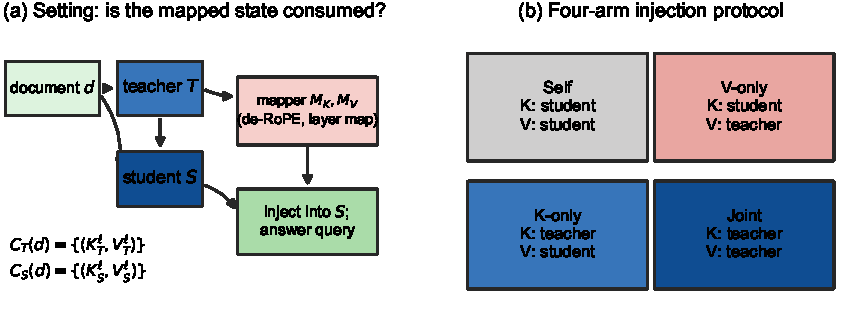
\includegraphics[width=\textwidth]{figures/fig_setting.pdf}
\caption{设定与协议。(a) 一份文档分别被教师与学生预填充；映射器把教师状态对齐到学生
空间（键在映射前先去 RoPE）。我们问的是该映射后的状态是否被\emph{消费}，而不只是它
是否可被线性预测。(b) 四臂协议。Self 是学生自身的缓存并作为参照；K-only 与 V-only 分别
隔离寻址与内容；Joint 是完整移交。}
\label{fig:setting}
\end{figure}

% ============================================================================
\section{相关工作}

\subsection{跨模型 KV 缓存传输}
\label{sec:rw-transfer}
最接近的一条工作线是跨模型映射 KV 状态。Heo 等人~\cite{heo2026crossmodel}提出了
一个闭式的逐头岭回归映射器，配合去 RoPE 的键与跨层源选择，用于模型家族内部的预填充
复用，并报告键比值的可预测性更高。Cache-to-Cache~\cite{fu2026c2c}在 LLM 之间传输
语义状态以实现直接通信；Mixture-of-Translators~\cite{lee2026translators}在异构 LLM 之间
翻译缓存；LatentAlign~\cite{dery2026latentalign}通过 KV 缓存对齐来对齐隐空间。这些系统
用人工设计的映射传输完整 KV 状态，并以 teacher-forced 似然或贪心重叠度来评测，我们的
出发点也是同一处：我们旧的评测器会在功能上并不存在迁移时报告看似存在的迁移，而仅有
teacher-forced 似然不足以证明功能性迁移。

大量同期文献在这一想法之上构建服务系统，报告的结果显著优于我们。
CacheBridge~\cite{cachebridge2026}把注意力校准的映射器与服务循环共同设计，在若干模型
家族上于 agent、对话、推理与检索负载中保留了大部分重填充任务质量；
ACCT~\cite{acct2026}把源缓存编译为稀疏的目标状态，在压缩 KV 预算下达到目标模型自身
推理的水平；CacheLink~\cite{cachelink2026}面向消费方行为学习键与值的联合修正，并明确
指出重建保真度是消费方效用的劣质代理；KV-Lingo~\cite{kvlingo2026}用对消费方自身预测的
蒸馏来训练逐层翻译器；BridgeKV~\cite{bridgekv2026}加入逐分量的非线性映射与第二阶段的
低秩适配；一个通用上下文复用层~\cite{contextreuse2026}在长上下文基准上报告优于原生目标
模型，并实现接近原生的跨家族交接；HeteroFold~\cite{heterofold2026}与
Swarm Telepathy~\cite{swarmtelepathy2026}实现跨模型家族的迁移；
RaReCache~\cite{rarecache2026}把残余差距归因于少数信息密集的位置并重算它们。
有两点把这条线同本文区分开。映射器是按消费方行为拟合的——通过蒸馏、通过行为目标、
通过非线性分量或通过可训练的修正阶段——而不是按状态距离拟合；质量是在通用的长上下文
与 agent 基准上、用较大的消费方模型度量的。我们把这些工作作为同期工作引用：它们出现于
本研究写作期间，我们不主张对其中若干工作同样具备的“消费空间”洞见拥有优先权，
第~\ref{sec:discussion-reconcile}~节讨论它们的结果与我们的结果何以能同时成立。

\subsection{什么才算迁移的证据}
\label{sec:rw-evidence}
本文的第一条贡献是一个评测主张，而它已经不再只属于我们。
一项因果审计~\cite{latentaudit2026}在消费方边界上以受控替代物替换发送方的消息，表明
聚合的任务效应并不能识别消费方是否使用了针对被评样本生成的内容。
PACT-Check~\cite{pactcheck2026}发现，训练出的桥接所带来的增益可以由无信息的发送方信号、
自我通信与仅训练消费方复现，并提出一种把它们分开的核算方法。
\cite{funccache2026}的 Functional Cache Divergence 表明，被复用的缓存可以在不复制原生
模型行为的情况下保留有用的任务信息，且首 token 一致并不意味着答案内容一致。
一项关于修复预算该花在哪里的研究~\cite{repairbudget2026}报告：一个远离完整预填充缓存的
重算缓存反而是更好的选择，该文称之为\emph{上下文兼容性}。
这些结果与我们的结果是从不同方向到达的同一个观察：交出去的状态值的是消费方拿它做什么，
而不是它像什么。我们保留自己的表述形式，是因为它在任务上而非在代理量上度量，是因为它
与第~\ref{sec:decomp}~节的四臂分解配套，也是因为我们的内容对照破坏的是键--值对应关系，
而不只是内容。

\subsection{KV 缓存优化}
\label{sec:rw-kvopt}
FlashAttention~\cite{dao2022flashattention}降低显存流量；投机解码
~\cite{leviathan2023fast,chen2023accelerating}降低延迟；KV 量化
（KIVI~\cite{kivi2024icml}、KVQuant~\cite{kvquant2024nips}）压缩缓存。这些工作都在单一
模型内部进行；我们研究的是状态本身被跨模型消费的过程。

\subsection{压缩、蒸馏、合并与拼接}
\label{sec:rw-merge}
量化~\cite{frantar2023gptq,dettmers2024qlora}、蒸馏
\cite{hinton2015distilling,touvron2023llama}、模型合并~\cite{ties2023merging,dare2024icml}
与模型拼接~\cite{bansal2021stitching}修改或合并权重。我们的消费适配器在精神上最接近
参数高效适配：它在预训练模型与状态映射器都冻结的情况下，只增加一个小的低秩模块。

\subsection{跨模型表示对齐}
\label{sec:rw-align}
“独立训练的神经网络会收敛到同一个表示、彼此只差一个简单映射”这一假设，就是柏拉图
表示假说（Platonic Representation Hypothesis）~\cite{prh2024}；相对表示
（relative representations）~\cite{relrepr2022}把它变成一个通信信道——用状态到一组共享
锚点的距离来表达该状态。模型拼接~\cite{bansal2021stitching}则确立了小的学习式接口可以
在功能上连接两个表示空间。
近期工作进一步澄清了收敛的是表示的哪一部分：一种“结构优先于几何”的论述
~\cite{structuregeo2026}主张收敛的是关系结构而不是坐标；MATCHA~\cite{matcha2026}
把层对应关系与特征映射联合学习，并报告层对应是多对多的“带”，而不是本文作为默认的
按相对深度成对的映射。
我们把这条文献读作支持而非否定我们的结论：共享或可线性映射的几何正是线性翻译器得以
存在的前提，而我们的发现是——这样的翻译器可以重建状态，而消费方仍然无法使用它。
收敛性结果所识别出的目标是结构；一次可用的交接所需要的目标是消费方自身的计算。

\subsection{注意力与位置结构}
\label{sec:rw-attn}
Transformer~\cite{vaswani2017attention}把键（寻址）与值（内容）分开；RoPE~\cite{su2024rope}
为键加入位置结构。我们在映射键之前剥离位置结构，并把消费方的路由
（$A=\mathrm{softmax}(QK^{\top})$）与输出通路（$O=AVW_O$）作为研究对象。

\paragraph{术语。}
本文命名三个量，它们不可互换。\emph{重建保真度}是映射后的状态与消费方自己会产生的那种
状态之间的距离。\emph{消费空间对齐}是在消费方从该状态计算出的量上拟合映射器——它的
注意力输出、它的 $o$ 投影，或它的下一 token 预测——而不是在状态本身上拟合。
\emph{功能兼容性}是消费方能够从交出的状态回答问题这一性质，也是我们的主指标所度量的东西。
同期工作使用\emph{上下文兼容性}~\cite{repairbudget2026}指一个相关但更窄的概念——
可用上下文对缓存中其他材料的依赖。

% ============================================================================
\section{方法}

\subsection{问题设定}
\label{sec:problem-setup}
给定教师 $T$ 与学生 $S$，层数分别为 $L_T$ 与 $L_S$。对一份文档 $d$，每个模型产生 KV
缓存 $C_m(d)=\{(K_m^\ell,V_m^\ell)\}_{\ell=1}^{L_m}$。映射器用层映射
$\pi:[L_S]\to[L_T]$（层数不等时按比例，层数相等时取恒等）把教师状态映射到学生空间。
键在映射前先做去 RoPE，映射后再施加学生的位置编码。映射后的文档状态被注入学生，而学生
在生成时只能看到问题；随后我们测量它是否能回答一个留出问题。

\subsection{注入协议}
\label{sec:injection}
每个评测样本从文档状态出发构造四个臂（图~\ref{fig:setting}b）：
\textbf{Self}（学生的 K 与 V）、\textbf{K-only}（映射后的教师 K 配学生的 V）、
\textbf{V-only}（学生的 K 配映射后的教师 V）与\textbf{Joint}（映射后的教师 K 与 V）。
Self 是参照：它度量学生在读取自身状态时的上限。K-only 与 V-only 分别隔离寻址与内容；
Joint 是完整移交。

\subsection{功能兼容性分解}
\label{sec:decomp}
设 $O_S=A_SV_SW_O^S$ 是学生读取自身缓存时的注意力输出，$\hat O=\hat A\hat VW_O^S$ 是它
读取被移交缓存时的输出，其中学生的输出投影 $W_O^S$ 冻结。该扰动可以精确拆分：
\begin{equation}
\hat O-O_S
= \underbrace{(\hat A-A_S)V_SW_O^S}_{\text{路由项}}
+ \underbrace{\hat A(\hat V-V_S)W_O^S}_{\text{消费项}} .
\label{eq:decomp}
\end{equation}
第~\ref{sec:injection} 节的四个臂开关这两个项。K-only 令 $\hat V=V_S$，只留下路由项；
V-only 令 $\hat A=A_S$，只留下消费项；Joint 同时携带两项及其交互。式~\eqref{eq:decomp}
是关于扰动的恒等式，而不是「任务性能可加性分解」的主张：精确匹配是输出的离散函数，而
似然尺度上的交互项在不同模型对之间会变号（附录~\ref{app:factorial}）。我们把它当作命名
两项兼容性要求的框架——接收方的路由必须能容纳被移交的键，其消费通路必须能接受被移交的
值——并通过干预、而不是算术来检验每一项要求。该恒等式说明了每个臂打开了哪一项，但它
并不说明哪一项限制了任务性能，因为这两个项是在一个并非任务指标的量纲（输出扰动）上
测量的。

\subsection{修正后的评测}
\label{sec:eval-protocol}
本工作早期版本所用实现在评分时让同一个缓存推进过提问\emph{与标准答案}，随后在这个被
改动的缓存上调用贪心生成，于是模型复述了它刚被展示的答案。第二个缺陷把最后的提问 token
重新作为生成的第一个输入，一旦缓存被扰动就会退化成标点循环。两个缺陷都在该实现中，
我们审计了它；我们没有审计第三方实现。我们采用的修正评测器要求 teacher-forced 对数
似然与贪心生成各自从\emph{全新}缓存开始，并且第一个生成 token 取自预填充的 logits。
我们在三种学生规模的完整 $56$ 题 Self 测试集上，用全前缀参考实现校验了修正评测器
（图~\ref{fig:evalcheck}）。归一化答案精确匹配在 $0.964$（$0.6$B）、$0.929$（$1.7$B）与
$0.982$（$4$B）的题目上一致，且每种学生最多相差两题；首 token top-1 一致率为 $0.929$、
$0.929$ 与 $0.982$；两条路径首 token 分布的中位 $KL$ 为 $0.0047$、$0.0015$ 与 $0.0010$
nats。token 级贪心一致率更低（$0.786$、$0.804$、$0.929$），因为贪心分词会漂移而不改变
抽取出的答案；最大绝对 logit 误差为 $1.344$、$0.875$ 与 $0.969$。我们对这一残差做了
归因，而不只是报告它。重复文档预填充是确定性的（缓存逐比特一致），并且当捕获到的缓存
被直接安装（而不是经由 numpy 往返）时、以及当提问的位置偏移被显式传入时，注入路径都
逐比特复现参考实现。剩下的是注意力内核路径本身——单 token 提问对接缓存 与 全序列预填充
之别——它解释了全部残差（在八题探针上最大绝对 logit 误差为 $0.844$、中位 $KL$ 为
$0.005$ nats），并且在 eager attention 下并不缩小。这些不一致是在 bf16 精度下被以不同
方式解决掉的近似平局，而不是缓存或位置处理方式的缺陷。同一校验器在第二个域上也成立
（第~\ref{sec:second-domain} 节）。

\begin{figure}[t]
\centering
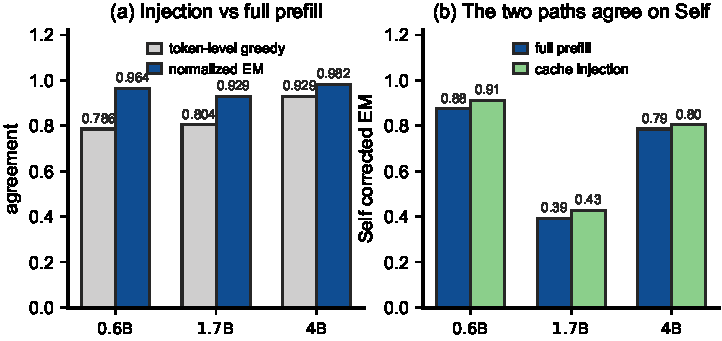
\includegraphics[width=0.86\textwidth]{figures/fig_evalcheck.pdf}
\caption{修正评测器的校验：在每种学生规模的完整 $56$ 题 Self 测试集上，缓存注入与全
前缀参考实现的对比，种子 0。(a) 两条路径的一致率。token 级贪心一致率低于归一化精确匹配
一致率，因为贪心分词会漂移而不改变抽取出的答案。(b) 第一个生成 token 的 logits 在绝对值
$1.344$ 以内一致，首 token top-1 一致率为 $0.93$--$0.98$，两条路径下的 Self 精确匹配至多
相差两题。一个归因探针把全部残差定位在注意力内核路径上：重复捕获、缓存往返与显式位置
偏移都是精确的。}
\label{fig:evalcheck}
\end{figure}

后文中的\emph{修正 EM}都指该评测器下的贪心精确匹配。本工作先前版本报告的所有 EM 数字
都由那条有缺陷的路径产生，均已撤回；修正说明与旧表作为补充材料提供。

\subsection{映射器}
\label{sec:mappers}
默认映射器是在标定数据上拟合的逐（层，头）仿射岭回归。我们另外为值定义了两个消费空间
映射器：(i) \textbf{注意力输出感知}映射器，在标定集上匹配 $A_S V_T \to A_S V_S$，即它在
学生读取值的位置上拟合；(ii) \textbf{$W_O$ 感知}映射器，它额外经过学生的输出投影，并对
每个 KV 头 $h$ 满足：对 GQA 组内的每个分组查询头 $q$，$M_h W_{O,q} \approx N_q$，其中
$N_q$ 是把 $A_q V_{T,h}$ 映射到 $A_q V_{S,h} W_{O,q}$ 的岭回归映射。目标被打乱的映射器
用\emph{另一份}文档的目标拟合同一目标函数，作为内容特异性对照。所有映射器都只在标定
划分上训练。

\subsection{消费适配器}
\label{sec:adapter}
为了检验接收模型是否能被变得兼容，我们在学生的注意力投影上加入秩 $r$ 的低秩修正
$\mathrm{proj}'(x)=Wx+B(Ax)$，其中 $B$ 初始化为零，并在注入映射后教师 KV 的条件下，
只用标定划分上的下一 token 交叉熵训练 $\{A,B\}$；学生与映射器冻结。除另有说明外，
$r=8$，被适配的模块是 \texttt{o\_proj}，优化器为 Adam、学习率 $10^{-3}$、训练 $20$ 轮，
梯度裁剪为 $1.0$。我们消融了被适配的投影以及适配器所训练的状态（教师、学生，或打乱
文档的教师 KV）。每种训练条件都从零训练自己的适配器，随后该单一适配器在全部四个注入臂
上评测；参数不跨条件共享。
% ============================================================================
\section{实验设置}

\subsection{模型与模型对}
\label{sec:models}
所有模型都来自 Qwen3 家族~\cite{qwen3report2025}：$0.6$B、$1.7$B、$4$B 与 $8$B 参数。$8$B 与 $4$B 模型有 $36$
层，$1.7$B 与 $0.6$B 模型有 $28$ 层；全部使用 $8$ 个键/值头、头维度 $128$，查询侧采用
分组查询注意力。我们评测所有「教师严格大于学生」的六个有序模型对：$8$B$\to0.6$B、
$4$B$\to1.7$B、$4$B$\to0.6$B、$8$B$\to1.7$B、$1.7$B$\to0.6$B 与 $8$B$\to4$B。其中两个
模型对层数相等（$8$B$\to4$B、$1.7$B$\to0.6$B），四个层数不等。

\subsection{数据}
\label{sec:data}
我们使用一个合成的域外（OOD）语料：把一张虚构实体构成的隐藏知识图谱渲染成项目状态
文档，问题按跳数 $1$--$4$ 采样，答案由程序校验。数据划分按实体簇进行（每个种子
$70$ 训练 / $28$ 验证 / $56$ 测试题），因此测试实体从不出现在训练中。测试问题来自
$8$ 份互不相同的文档（每份文档约七题），所以我们对对照套件报告以文档为聚类单位的
bootstrap 区间，并在解释逐样本区间时考虑这一聚类结构。作为第二个域，我们在 SQuAD 上
评测（$n=30$ 个留出问题），其映射器只在合成的 OOD 训练划分上标定。

\subsection{指标与对照}
\label{sec:metrics}
我们的主任务指标是修正后的贪心精确匹配。teacher-forced 答案对数似然（LL）相对同一样本的
Self 臂报告，它是一个次要的、明确非任务性的量。内容对照包括：错误文档缓存（另一个项目
的状态）、逐层矩匹配的随机高斯键、随机 KV 对、全零缓存、恒等（未映射）的 V-only 注入，
以及学生自身缓存的两种\emph{破坏对应关系}的置换：一种置换键的 token 顺序而让值留在原位，
另一种是它在值上的镜像。我们还计算了一个「同一置换」臂，它同时重排键与值；我们只把它
作为不变性检查来报告，因为注意力对 $K$ 与 $V$ 的共同重排是不变的，这种臂无法检出内容
损坏。其他所有对照都会破坏内容。这些置换作用于学生自身的状态，因此按构造它们与模型对
无关，它们在模型对之间的一致性属于自洽性检查，而不是独立结果。对适配器，我们还额外在
学生 KV 与打乱文档的教师 KV 上训练。

\subsection{统计协议}
\label{sec:stats-protocol}
本文中的每一次比较都跑三个种子（0、1、2），每个种子有自己的实体簇划分。所有主要量都
报告种子间的均值 $\pm$ 标准差。臂间差异的显著性用同一批样本上相对 Self 的配对 Wilcoxon
符号秩检验评估，在报告逐样本区间处使用以文档为聚类单位的 bootstrap CI95。我们只在相应
报告给出 $p$ 值的地方报告 $p$ 值，并指出它对应的种子或种子聚合。

\subsection{验证性与探索性分析}
\label{sec:analyses}
我们明确区分这两类，因为指标修正改变了我们自己部分早期工作的地位。

\emph{验证性。} 四臂注入协议、六个模型对、三种子要求与预注册的 G0 门限早于本次修订。
内容对照套件、层映射消融、留出层扫描、路由/映射器比较、评测器校验、修复态下的层打乱、
适配器因果性检验、跨域修复尝试、路由感知键映射器、映射器目标扫描与标定混合对照，都在
相应实验运行之前就已在书面修订计划中连同判定规则一并指定；该计划与原始报告都在仓库中。

\emph{探索性。} 修正评测器、消费适配器、投影消融、把似然增益分解为 K 与 V 主效应及其
交互（附录~\ref{app:factorial}），以及「只有等深模型对才有非零 V-only EM」这一观察，
都引入于我们发现评测器缺陷之后。它们属于产生假设的分析。我们早先的两个结论也发生了
变化：层映射打乱，我们曾报告为无害，在映射器被修正后是有害的（第~\ref{sec:layer-align} 节）；
旗舰对上适配器的行为也弱于等深对。

\emph{已撤回。} 我们预注册的 G0 门限定义在有缺陷的 EM 指标上，用的是更早的标定/评测
划分（$42$/$14$），当时 V-only 在答案似然上比 Self 高 $+1.75$（$-9.97 \pm 2.60$ 对
$-11.72 \pm 2.07$，95\% 区间重叠）。因此它的任务指标条款被撤回。在修好基线重复计数
缺陷之后，我们在当前划分（$70$/$56$）上重跑了它的似然条款，结果 V-only 在每个种子上
都等于或低于 Self（$\dll = -0.045$、$-0.219$、$-0.415$；$p = 0.024$、$0.125$、
$0.144$，均不显著）。该条款的结论——V-only 不迁移——没有改变，但它建立在预注册检验的
重跑而不是原始运行之上；它也不能再被读作关于任务性能的陈述。

% ============================================================================
\section{结果}

\subsection{教师状态不能回答问题}
\label{sec:teacher-states}
表~\ref{tab:main} 与图~\ref{fig:fourarm} 报告了六个模型对在三个种子上的修正 EM 与 LL。
LL 的增量与已发表数值完全一致（例如 $8$B$\to0.6$B 的 K-only $+2.62$、V-only $-0.23$），
这确认了流水线本身没有变化，只是 EM 路径坏了。

学生用自己的缓存能答对大部分问题（学生为 $0.6$B 的三个模型对为 $0.899 \pm 0.010$，
学生为 $1.7$B 的两个模型对为 $0.440 \pm 0.010$，学生为 $4$B 的为 $0.815 \pm 0.021$）。
没有任何教师臂接近这一水平。在种子上平均后，K-only 至多 $0.149 \pm 0.010$
（$8$B$\to4$B），Joint 至多 $0.065 \pm 0.055$（$8$B$\to4$B）；任一种子上单个臂达到
的最大值是 $0.161$（K-only）与 $0.125$（Joint），都出现在 $8$B$\to4$B 上。在旗舰的
$8$B$\to0.6$B 对上，三个教师臂在每个种子上都是 $0.000$。唯一超过 $0.15$ 的臂是
$8$B$\to4$B 上的 V-only，为 $0.440 \pm 0.010$——略高于该对 Self（$0.815$）的一半——
而 V-only 在四个层数不等的模型对上都是 $0.000$。在种子上平均后，没有其他教师臂超过
$0.15$。以文档为重采样单位（每个种子八个簇），该对的 V-only 臂在三个种子上的 CI95 为
$[0.375, 0.482]$、$[0.429, 0.482]$ 与 $[0.429, 0.482]$：每个区间都排除零，且都远低于
同一种子的 Self（$0.804$--$0.839$）。同样的重采样使 K-only 落在 $[0.071, 0.250]$ 之内、
Joint 不超过 $0.179$，因此聚类只是加宽了区间，没有改变任何臂的排序。

与此同时，同样的注入显著抬高了 teacher-forced 似然：K-only 最多 $+8.52$
（$8$B$\to4$B），Joint 最多 $+8.37$，旗舰对为 $+2.62$ 与 $+4.52$。图~\ref{fig:fourarm}
直接展示了这种分离：把似然抬高最多的臂并不是能回答问题的臂。

\begin{table}[t]
\centering
\small
\caption{修正后的四臂扫描，六个模型对，三个种子，$n=56$。EM 是修正后的贪心精确匹配；
$\dll$ 是相对 Self 的 teacher-forced 答案对数似然。数值为种子间的均值 $\pm$ 标准差。
标准差留空表示来源未报告该单元格的离散度；每一个这样的单元格在三个种子上都是 $0.000$
的臂。EM 的文档聚类 CI95（聚类 $=$ 文档，每种子八个）由归档的逐样本行对每个种子分别计算，
并在正文中给出那些有结论依赖的臂的区间。}
\label{tab:main}
\begin{tabular}{lcccccccc}
\toprule
 & & \multicolumn{4}{c}{修正 EM} & \multicolumn{3}{c}{相对 Self 的 $\dll$} \\
\cmidrule(lr){3-6}\cmidrule(lr){7-9}
模型对 & Self & K & V & J & K & V & J \\
\midrule
$8$B$\to0.6$B   & $0.899{\pm}0.010$ & $0.000$ & $0.000$ & $0.000$ & $+2.62{\pm}0.29$ & $-0.23{\pm}0.19$ & $+4.52{\pm}0.15$ \\
$4$B$\to1.7$B   & $0.440{\pm}0.010$ & $0.054{\pm}0.018$ & $0.000$ & $0.024{\pm}0.010$ & $+2.90{\pm}0.09$ & $+2.91{\pm}0.21$ & $+2.31{\pm}0.25$ \\
$4$B$\to0.6$B   & $0.899{\pm}0.010$ & $0.000$ & $0.000$ & $0.006{\pm}0.010$ & $+1.58{\pm}0.02$ & $-1.22{\pm}0.05$ & $+2.50{\pm}0.52$ \\
$8$B$\to1.7$B   & $0.440{\pm}0.010$ & $0.000$ & $0.000$ & $0.012{\pm}0.021$ & $+1.04{\pm}1.53$ & $+5.63{\pm}0.04$ & $+4.69{\pm}0.27$ \\
$1.7$B$\to0.6$B & $0.899{\pm}0.010$ & $0.030{\pm}0.010$ & $0.113{\pm}0.052$ & $0.000$ & $-0.82{\pm}0.02$ & $+0.63{\pm}0.17$ & $-2.25{\pm}0.14$ \\
$8$B$\to4$B     & $0.815{\pm}0.021$ & $0.149{\pm}0.010$ & $0.440{\pm}0.010$ & $0.065{\pm}0.055$ & $+8.52{\pm}0.28$ & $+2.52{\pm}0.07$ & $+8.37{\pm}0.28$ \\
\bottomrule
\end{tabular}
\end{table}

\begin{figure}[t]
\centering
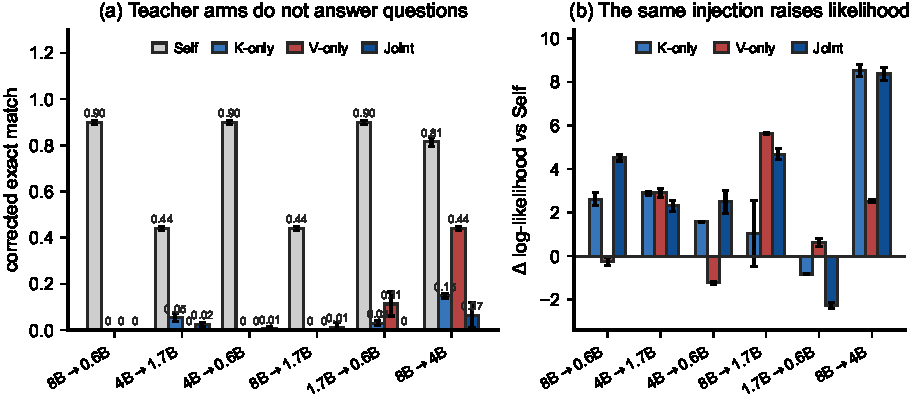
\includegraphics[width=\textwidth]{figures/fig_fourarm.pdf}
\caption{修正后的四臂扫描（三个种子）。(a) 只有学生自身的缓存能回答问题；未标注的柱为
$0.00$。(b) 同样的注入抬高了 teacher-forced 似然，且在没有产生任何答案的地方最明显。
误差棒为来源报告了离散度时的种子间标准差。}
\label{fig:fourarm}
\end{figure}
\subsection{似然增益与内容无关}
\label{sec:controls}
一个只看似然的协议会读作「迁移」的那些似然增益，并不携带文档内容（表~\ref{tab:controls}、
图~\ref{fig:controls}）。在三个种子上，错误文档缓存——另一个项目的状态——让 K-only 似然
增益基本不变（$+2.61 \pm 0.31$ 对 $+2.62 \pm 0.29$）；逐层矩匹配的随机高斯键复现了
$89\%$（$+2.33 \pm 0.27$）；全零缓存复现了 $105\%$（$+2.75 \pm 0.01$），超过了真实的
K-only 注入；联合臂的行为相同（错误文档 $+4.50$ 对真实 $+4.52$）。在来源报告了文档聚类
区间的种子 0 上，K-only 增益的 CI95 为 $[+2.21, +2.64]$、全零 KV 增益为
$[+2.49, +3.00]$，因此对照的区间与真实臂的区间重叠。

这些臂中的每一个都给出接近或等于 $0$ 的修正 EM。一个确实破坏对应关系的对照则很
有信息量：置换学生自身键的 token 顺序、同时让值仍与其位置对齐，会在三个种子上把 EM 压到
$0.000$，值上的镜像对照同样如此（表~\ref{tab:controls}）。先前草稿所依赖的「同一置换」
臂并不是内容对照——注意力对 $K$ 与 $V$ 的共同重排是不变的——它在各种子上返回 $0.929$、
$0.875$ 与 $0.857$，正是该不变性所预测的；我们只把它作为一个检查来报告，即评测器没有
抑制某个置换不变量。

因此评测器对上下文并非不敏感：它在学生自身缓存上得 $0.899 \pm 0.010$，对教师注入的状态
什么也不返回，键--值对应被破坏时也什么也不返回。对等深模型对 $1.7$B$\to0.6$B，同样的
模式在三个种子上成立。在那里，真实的 K-only 注入\emph{降低}了答案似然
（$-0.82 \pm 0.02$），并答对 $0.030 \pm 0.010$ 的问题，而无内容的缓存抬高了它
（全零 KV $+2.75 \pm 0.01$，随机 K $+2.33 \pm 0.27$，错误文档 K $-0.78 \pm 0.06$），
最多答对 $0.036$；错误文档缓存在两个轴上都与真实缓存无法区分。这里这种分离是反方向的
——似然随内容被破坏而提高——这是从另一侧看到的同一个似然指标失效。不过与 $8$B 不同的
是，无内容臂并非在每一次比较中都超过真实臂，而且无内容臂按构造与模型对无关，所以我们把
$1.7$B 这套结果读作对 $8$B 对照的佐证，而不是独立复现。

\begin{table}[t]
\centering
\small
\caption{$8$B$\to0.6$B 上的内容对照，修正评测器，三个种子（均值 $\pm$ 标准差）。
「Share」是该臂的 $\dll$ 除以同一批 run 的 K-only $\dll$。最后三行作用于学生自身的
缓存而不是教师状态，因此按构造在每个模型对上都相同；前五行是教师臂或无内容臂。}
\label{tab:controls}
\begin{tabular}{lccc}
\toprule
臂 & 相对 Self 的 $\dll$ & 修正 EM & 占 K-only 增益的比例 \\
\midrule
K-only（真实）          & $+2.62{\pm}0.29$ & $0.000$ & $100\%$ \\
错误文档 K              & $+2.61{\pm}0.31$ & $0.000$ & $100\%$ \\
随机高斯 K              & $+2.33{\pm}0.27$ & $0.012{\pm}0.010$ & $89\%$ \\
全零 KV                 & $+2.75{\pm}0.01$ & $0.000$ & $105\%$ \\
Joint（真实）           & $+4.52{\pm}0.15$ & $0.000$ & --- \\
错误文档 Joint          & $+4.50{\pm}0.18$ & $0.000$ & --- \\
\midrule
打乱 K（学生）          & $-1.19{\pm}0.10$ & $0.000$ & --- \\
打乱 V（学生）          & $-1.28{\pm}0.04$ & $0.000$ & --- \\
对 K 与 V 施加同一置换（学生） & $-0.01{\pm}0.00$ & $0.887{\pm}0.037$ & --- \\
\bottomrule
\end{tabular}
\end{table}

\begin{figure}[t]
\centering
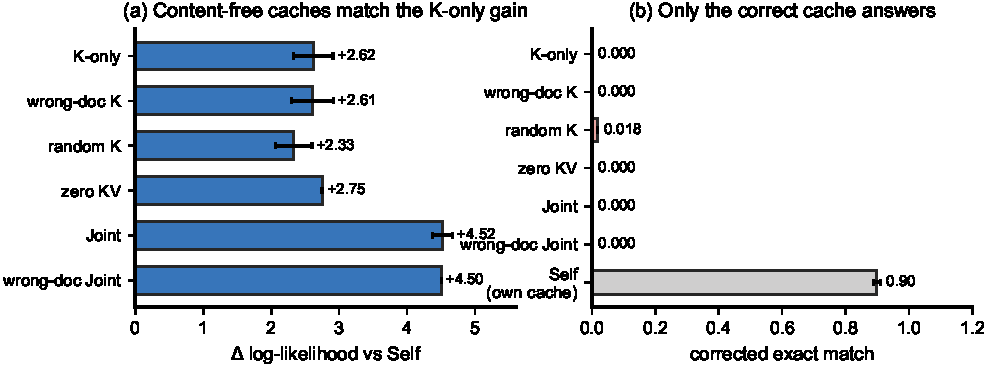
\includegraphics[width=\textwidth]{figures/fig_controls.pdf}
\caption{$8$B$\to0.6$B 上的内容对照。(a) K-only 与 Joint 的似然增益被错误文档、随机与
全零缓存追平或超过。(b) 没有任何教师臂或无内容臂能回答问题，而学生自身缓存得 $0.899$。
评测器能读出可用上下文，对注入状态返回空。误差棒为报告了离散度时的种子间标准差。}
\label{fig:controls}
\end{figure}

\subsection{第二个域}
\label{sec:second-domain}
在 SQuAD 上，映射器只在合成 OOD 划分上标定、$n=30$ 个留出问题，修正 EM 在三个种子上
都是 Self $0.367$，而 K-only、V-only 与 Joint 均为 $0.000$。校验器在这里未经修改地重复：
在这 $30$ 个 Self 题上归一化 EM 一致率为 $0.933$，首 token top-1 一致率为 $0.933$，中位
$KL$ 为 $0.005$ nats，两条路径下 Self 的精确匹配完全相同。K-only 似然增益在三个种子上
平均为 $+5.24$（种子 0 为 $+5.223$，该种子下相对 Self 的 Wilcoxon $p = 2.8\times10^{-6}$；
V-only $+1.053$，$p=0.205$；Joint $+3.497$，$p=1.9\times10^{-4}$）。K-only 增益在每个
种子上都显著（$0$--$2$ 号种子的 $p = 2.8\times10^{-6}$、$4.7\times10^{-7}$、
$2.1\times10^{-7}$）；我们报告这些逐种子检验而不是合并的 $p$ 值，因为合并检验所需的
逐样本增量没有被保留。因此该负结果与 LL/EM 的分离在域外、在映射器从未见过的数据上复现。
两种修复都不能迁移到这套数据：在合成域上训练的映射器与适配器在这里都让 K-only 与联合臂
EM 停在 $0.000$（第~\ref{sec:adapter-results} 节、表~\ref{tab:squadrepair}）。我们注意到，
旧评测器在这套数据上给 K-only 打了 $0.733$ EM，而修正评测器给它 $0.000$；旧的 Self 分数
为 $0.767$，修正后的 Self 为 $0.367$：该缺陷既移动了臂，也移动了参照点。当修复在此域内
重新拟合时该域是否也会失败，是第~\ref{sec:adapter-results} 节回答的问题，也正是它使兼容性
成为任务条件性的、而非模型对的性质。

% ============================================================================
\section{分析}

\subsection{一旦消费者能读取状态，层对齐就变得重要}
\label{sec:layer-align}
对等深模型对 $1.7$B$\to0.6$B，我们只改变层映射并保持能力差距不变
（图~\ref{fig:layers}a）。在早先工作使用的仿射映射器下，值臂被钉在地板上，层映射看起来
无关紧要：按比例（恒等）映射在三个种子上给出的修正 V-only EM 为 $0.05$--$0.14$，
$\pm3$ 的偏移与随机置换在每个种子上都给出 $0.000$，置换甚至\emph{抬高}了 V 的似然增量
（种子 0 为 $+1.35$ 对 $+0.83$）。我们曾把这读作层对齐不重要。这是映射器的地板效应：
值臂已经在 $0$ 上时，任何层映射都无法让它更差。

用表~\ref{tab:mappers} 的消费空间映射器重复这一消融，答案就变了：它把按比例映射的
V-only EM 在三个种子上抬到 $0.911/0.929/0.964$（均值 $0.935$）。在种子 0 上，同样的偏移
与置换现在要付出大部分迁移：V-only EM 降到 $0.214$（偏移 $+3$）、$0.232$（偏移 $-3$）与
$0.107$（随机置换）。每个被打乱的臂都低于按比例映射中最低的那个种子，并且种子 0 的
文档聚类区间把按比例臂（$[0.839, 0.982]$）与三个被打乱的臂（$[0.125, 0.304]$、
$[0.143, 0.321]$、$[0.054, 0.179]$）分开。因此层对齐是必要的、但不是充分的。在映射器
未能把值放到消费者读取它的位置时，层对齐是不可见的；一旦映射器做到这一点，它就变成
主导因素。

对层数不等的模型对 $8$B$\to0.6$B，按比例映射给出最好且最稳定的联合似然（各种子上
$+4.41$--$+4.68$），而偏移、置换以及由标定学出的 top-1 源层选择都会降低它并且不稳定。
在这些替代层映射下，除一个学出的选择单元格（$0.107$）外，修正 V-only EM 在每个单元格
上都是 $0.000$，K-only 也从未超过 $0.179$。改进层映射并不能在这个模型对上创造出迁移。
我们不把这读作「对齐在这里不重要」，因为消费侧映射器在这个模型对上只能恢复 Self 的
四分之一（表~\ref{tab:mappers}）：同样的地板效应很可能仍然适用。修复态下的打乱实验只在
等深模型对上跑了。

由于修正 EM 在每个教师臂上都处于地板，四臂设计也可以在似然尺度上分解。我们在
附录~\ref{app:factorial} 中报告该分解与旗舰对上的 K 对 V 配对检验，但不作功能性解读：
K$\times$V 交互项在不同模型对之间变号，而第~\ref{sec:controls} 节表明，一个不携带任何
内容的缓存也能复现似然增益。

\subsection{两类彼此独立的失败：映射后的键扰动路由，映射后的值必须可被消费}
\label{sec:two-failures}
我们比较学生在自身键下与在映射后教师键下的注意力图（图~\ref{fig:mappers}b）。平均 top-1
文档 token 一致率在 $1.7$B$\to0.6$B 上是 $0.70$、在 $8$B$\to0.6$B 上是 $0.59$，且这些
数值在种子间稳定（$0.698$--$0.701$ 与 $0.577$--$0.590$）；路由全变差在种子上平均为
$0.167$ 与 $0.251$，而注意力\emph{分布}仍保持接近（余弦 $0.97$ 与 $0.93$）。因此映射后的
教师键保留了注意力分布的总体形状，却改变了每个提问最关注哪个文档 token，并且在大差距
模型对上改变更大。

在学生的读取值的位置拟合值映射器，可以恢复大部分 V-only 迁移（表~\ref{tab:mappers}、
图~\ref{fig:mappers}a）。对 $1.7$B$\to0.6$B，V-only EM 从 $0.113$（仿射）升到 $0.935$
（注意力输出感知）与 $0.899$（$W_O$ 感知），而 Self 为 $0.899$。对 $8$B$\to0.6$B，它从
$0.000$ 升到 $0.250 \pm 0.018$ 与 $0.268 \pm 0.018$，而 Self 为 $0.899$：同一个目标函数
在旗舰对上恢复了约四分之一 Self。目标被打乱的对照用另一份文档的目标拟合同一目标函数，
它停在地板附近（$0.077$ 与 $0.065 \pm 0.027$），因此这一恢复与该文档的内容绑定，而不是
对缓存的一般性变换。

值臂与键臂因为不同原因失败，四臂设计让两者保持分开。在值臂中，学生读取的是自身键，
因此它的路由就是学生自己的路由：失败在于映射后的值在表示空间中接近 $V_S$，而接收方
实际消费的量是 $A_S V W_O$。所以旗舰对上的残余缺口是接收方消费空间中的对齐缺口，而不是
寻址效应：这个臂从不接触映射后的键。在键臂中，以及继承了二者的联合臂中，学生被要求读取
教师键，其路由确实移动了（top-1 一致率在 $1.7$B$\to0.6$B 上为 $0.70$、在
$8$B$\to0.6$B 上为 $0.59$，注意力余弦为 $0.97$ 与 $0.93$）。我们把路由分歧作为键侧的
诊断量报告，把消费空间对齐作为值侧起作用的自变量，不再用其中一方去解释另一方。

我们还对键侧做干预，而不只是测量它（表~\ref{tab:routingkey}）。该干预用学生的注意力
质量重新加权同一个逐（层，头）岭回归拟合，使得精度被要求在学生真正关注的地方；在单位
权重下它精确复现仿射键拟合（全部六个 run 上 $\max|\Delta| = 0$）。它把路由分歧在
$1.7$B$\to0.6$B 上从 $0.167$ 压到 $0.139$（$17\%$）、在 $8$B$\to0.6$B 上从 $0.254$ 压到
$0.153$（各种子上 $38$--$43\%$），并把 top-1 一致率从 $0.70$ 提到 $0.87$、从 $0.58$ 提到
$0.84$。任务臂并没有跟着走：K-only EM 仍在地板上（路由感知映射器本身至多 $0.054$，
任何 run 中四个键臂合计至多 $0.089$，而学生自身缓存为 $0.899$），并且把同一目标函数拟合
到打乱文档的目标上——它不可能携带内容——在任务臂上并不更差（$8$B$\to0.6$B 上 $0.042$ 对
$0.030$），同时在 $1.7$B$\to0.6$B 上复现了似然增益（$+3.85$ 对 $+3.79$）。因此弥合路由
差距是一个我们能改变、却不能修复该臂的条件；我们据此把它称为针对「键侧可在路由空间中
修复」的负干预，而不是一次挽救，这也正是我们最终找到的修复位于消费侧的原因。

\begin{table}[t]
\centering
\small
\caption{路由感知键映射器与仿射键映射器的对比：三个种子，每种子 $56$ 个留出问题，
似然为平均答案对数似然相对学生自身缓存之差，路由 TV 为学生在映射后教师键下与在自身键下
路由之间的全变差距离，top-1 为文档 token 一致率。「routing」是路由感知映射器，
「routing-shuf」是把同一目标函数拟合到另一份文档目标上的版本。路由分歧移动了，任务臂
没有，且打乱对照并不更差。}
\label{tab:routingkey}
\begin{tabular}{llcccc}
\toprule
模型对 & 键映射器 & $\dll$ & EM & 路由 TV & top-1 \\
\midrule
$1.7$B$\to0.6$B & 仿射        & $-0.82$ & $0.030$ & $0.167$ & $0.700$ \\
$1.7$B$\to0.6$B & routing       & $+3.79$ & $0.000$ & $0.139$ & $0.872$ \\
$1.7$B$\to0.6$B & routing-shuf  & $+3.85$ & $0.006$ & $0.205$ & $0.842$ \\
$1.7$B$\to0.6$B & 原始层        & $+0.31$ & $0.030$ & $0.170$ & $0.745$ \\
\midrule
$8$B$\to0.6$B & 仿射          & $+2.62$ & $0.000$ & $0.254$ & $0.581$ \\
$8$B$\to0.6$B & routing         & $+2.26$ & $0.030$ & $0.153$ & $0.839$ \\
$8$B$\to0.6$B & routing-shuf    & $+1.35$ & $0.042$ & $0.214$ & $0.813$ \\
$8$B$\to0.6$B & 原始层          & $-0.98$ & $0.000$ & $0.773$ & $0.032$ \\
\bottomrule
\end{tabular}
\end{table}

表~\ref{tab:errorbudget} 把两个候选对齐目标与任务指标并置，对同样的五个映射器变体，
在共享 $0.6$B 学生的两个模型对（$1.7$B$\to0.6$B 与 $8$B$\to0.6$B；六个 run）上合并。
原始表示误差无法给它们排序：仿射映射器的原始误差远小于其他变体（$0.267$），EM 却排
倒数第二（$0.057$），而两个消费空间映射器带有 $0.70$--$0.77$ 的原始误差——是前者的两倍
多——却达到 $0.586$--$0.592$。在学生读取状态处测量的误差则能排序：注意力输出误差从
$3.20$（仿射）降到 $0.073$，$o$ 投影误差从 $3.75$ 降到 $0.081$。

五个变体太少，不足以据此立一条规则，所以我们改为扫描目标函数。令
$\mathcal{L}_\alpha = (1-\alpha)\|\hat V - V_S\|^2 +
\alpha\|A_S\hat V - A_S V_S\|^2$，$\alpha \in \{0, 0.1, \dots, 1\}$、
岭参数 $\lambda \in \{10^{-4}, 10^{-3}, 10^{-2}\}$，其中 $\alpha=0$ 精确复现仿射映射器、
$\alpha=1$ 精确复现注意力输出感知映射器；每个 run 在同样的留出问题上评出 $33$ 个配置，
在两个模型对与三个种子上共 $198$ 个点（表~\ref{tab:sweep}、图~\ref{fig:sweep}）。网格
确认了这一排序并让它更锐利。消费空间误差与 EM 呈强负秩相关，其 bootstrap 区间在每个 run
内都与原始误差区间不相交（$1.7$B$\to0.6$B 内注意力输出误差 $\rho=-0.964$
$[-0.983,-0.925]$、$o$ 投影误差 $-0.962$；$8$B$\to0.6$B 内 $-0.919$ 与 $-0.918$；
全部 $198$ 点上 $-0.799$ 与 $-0.823$）。原始表示误差不只是没有信息量：在每一个 run 内它
都与 EM\emph{正}相关（$8$B$\to0.6$B 上 $+0.890$ 到 $+0.944$，$1.7$B$\to0.6$B 上 $+0.934$
到 $+0.989$），因此状态空间误差最小的配置恰恰是回答问题最少的配置——这就是上面五个变体的
观察在更高分辨率下的形态。全部 $198$ 点上唯一的合并原始数值 $-0.27$ 之所以方向相反，
只是因为两个模型对的尺度不同（$8$B 对同时有更大的误差和更低的 EM），而且它仍远弱于消费
空间的数值。因此我们在网格支持的层面陈述这条规则：预测迁移的误差，是接收方在它消费该
状态的位置上对其所犯的误差，而不是状态之间的距离。有一个变体是真正的例外，我们如实
报告：目标被打乱的映射器在对着错误文档的目标时达到很低的注意力输出误差（$0.90$），
却只答对 $0.071$ 的问题，因为它拟合的量并不是答案所依赖的量。在拟合正确目标的映射器
族内，接收方读取状态处的对齐才跟随任务性能；原始表示误差不跟随。

\begin{table}[t]
\centering
\small
\caption{映射器目标扫描中每种误差度量与修正 V-only EM 的秩相关：每个 run $33$ 个配置，
两个模型对与三个种子共 $198$ 个点，相关与区间用平均秩计算（配置级 bootstrap）。在每一个
run 内原始误差都与 EM 正相关，因此它无法按任务性能给配置排序，而消费空间误差则是强负
相关。$198$ 点的合并值为：$e_{\text{raw}}$ $-0.267$ $[-0.373,-0.148]$、$e_{\text{attn}}$
$-0.799$ $[-0.846,-0.740]$、$e_{W_O}$ $-0.823$ $[-0.865,-0.770]$；只有合并的原始值是
负的，而它是模型对之间的量纲假象。}
\label{tab:sweep}
\begin{tabular}{lccc}
\toprule
误差度量 & $1.7$B$\to0.6$B & $8$B$\to0.6$B & 合并（$198$ 点） \\
 & 每个 run（各 $33$ 个） & 每个 run（各 $33$ 个） & \\
\midrule
$e_{\text{raw}}$  & $+0.93$ 到 $+0.99$ & $+0.89$ 到 $+0.94$ & $-0.267$ \\
$e_{\text{attn}}$ & $-0.99$ 到 $-0.93$ & $-0.95$ 到 $-0.90$ & $-0.799$ \\
$e_{W_O}$         & $-0.99$ 到 $-0.93$ & $-0.95$ 到 $-0.90$ & $-0.823$ \\
\bottomrule
\end{tabular}
\end{table}

\begin{figure}[t]
\centering
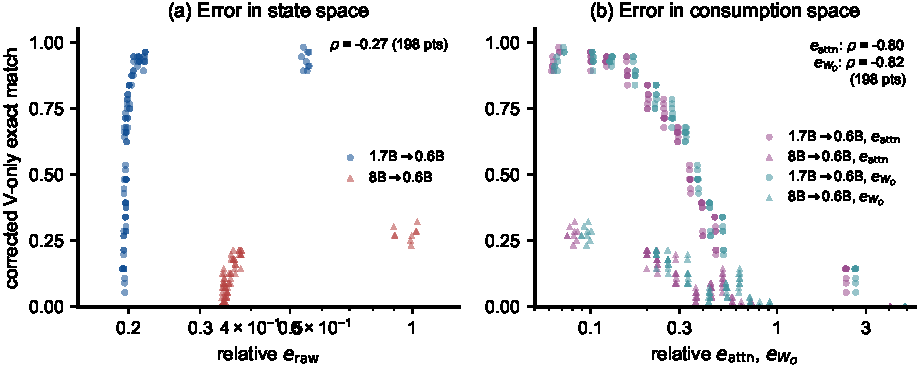
\includegraphics[width=\textwidth]{figures/fig_sweep.pdf}
\caption{映射器目标扫描，$198$ 个配置。每个点是一个 $(\alpha,\lambda)$ 设置，在同样的
留出问题上评分；横轴为对数刻度。(a) 状态空间误差：原始表示误差无法按任务性能给配置排序，
并且在每个模型对内都与任务性能正相关。(b) 消费空间误差：注意力输出与 $o$ 投影误差都先
下降若干数量级，EM 才上升，且它们在每个 run 内与 EM 的秩相关都是强负的。秩相关使用平均秩；
合并值见表~\ref{tab:sweep}。}
\label{fig:sweep}
\end{figure}

\begin{table}[t]
\centering
\small
\caption{同样这些映射器变体的状态空间误差与消费空间误差，在 $1.7$B$\to0.6$B 与
$8$B$\to0.6$B 及三个种子上合并。相对 Frobenius 误差，越小越接近：$e_{\text{raw}}$ 比较
映射后的 $V$ 与学生的 $V$，$e_{\text{attn}}$ 比较学生的注意力输出 $A_S V$，$e_{W_O}$
比较该输出经学生自身 $o$ 投影之后的结果。EM 为修正 V-only EM。与 EM 的秩相关在五个映射器
变体、六个 run 的合并均值上计算，并报告其逐 run 范围：$e_{\text{raw}}$ 为 $-0.10$
$[[-0.60,+0.05]]$，$e_{\text{attn}}$ 为 $-1.00$ $[[-1.00,-0.80]]$，$e_{W_O}$ 为 $-0.80$
$[[-1.00,-0.80]]$。五个变体与六个 run 太少，不足以给出 $p$ 值，因此表~\ref{tab:sweep}
与图~\ref{fig:sweep} 在映射器目标的 $198$ 个配置上重复该比较。}
\label{tab:errorbudget}
\begin{tabular}{lcccc}
\toprule
映射器 & $e_{\text{raw}}$ & $e_{\text{attn}}$ & $e_{W_O}$ & V-only EM \\
\midrule
原始层选择    & $3.73$ & $3.72$ & $3.65$ & $0.000$ \\
仿射                 & $\mathbf{0.267}$ & $3.20$ & $3.75$ & $0.057$ \\
注意力输出感知 & $0.772$ & $0.073$ & $0.082$ & $\mathbf{0.592}$ \\
打乱目标        & $5.58$ & $0.903$ & $1.09$ & $0.071$ \\
$W_O$ 感知            & $0.699$ & $\mathbf{0.076}$ & $\mathbf{0.081}$ & $0.586$ \\
\bottomrule
\end{tabular}
\end{table}

\begin{table}[t]
\centering
\small
\caption{值映射器目标与修正 V-only EM（三个种子，来源报告了离散度时为均值 $\pm$ 标准差）。
「Shuffled」是拟合到错误文档目标的同一目标函数。两个模型对的 Self 都是 $0.899 \pm 0.010$
（表~\ref{tab:main}）。在种子 0，仿射基线在 $1.7$B$\to0.6$B 上为 $0.054$、在
$8$B$\to0.6$B 上为 $0.000$。}
\label{tab:mappers}
\begin{tabular}{lcccc}
\toprule
模型对 & 仿射 & 注意力输出感知 & 打乱目标 & $W_O$ 感知 \\
\midrule
$1.7$B$\to0.6$B & $0.113$ & $\mathbf{0.935}$ & $0.077$ & $0.899$ \\
$8$B$\to0.6$B   & $0.000$ & $0.250{\pm}0.018$ & $0.065{\pm}0.027$ & $\mathbf{0.268{\pm}0.018}$ \\
\bottomrule
\end{tabular}
\end{table}

\begin{figure}[t]
\centering
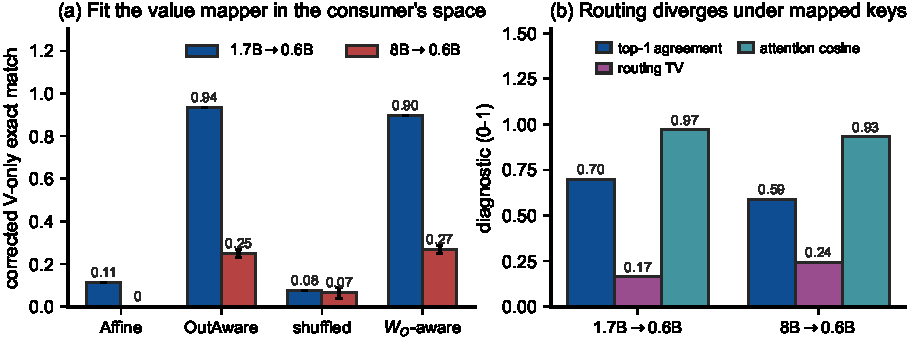
\includegraphics[width=\textwidth]{figures/fig_mappers.pdf}
\caption{(a) 按映射器目标给出的修正 V-only EM。在消费者空间中拟合映射器，可以在等深模型对
上恢复大部分值臂、在旗舰对上恢复约四分之一；打乱目标对照仍停在地板附近。(b) 相同模型对
的路由诊断：注意力余弦很高，而 top-1 一致率明显更低，且在大差距模型对上路由全变差更大。
top-1 一致率在种子间波动于 $0.698$--$0.701$（$1.7$B）与 $0.577$--$0.590$（$8$B）。}
\label{fig:mappers}
\end{figure}

\subsection{一个消费适配器恢复迁移}
\label{sec:adapter-results}
现在我们适配消费者而不是状态（表~\ref{tab:adapter}、图~\ref{fig:adapter}）。对学生输出
投影的秩 8 修正，在标定的教师 KV 上训练，把 $1.7$B$\to0.6$B 的 K/V/联合臂 EM 从
$0.030/0.113/0.000$ 提到 $0.940/0.940/0.827$，把 $8$B$\to0.6$B 的从
$0.000/0.000/0.000$ 提到 $0.792 \pm 0.162/0.357 \pm 0.047/0.470 \pm 0.119$。在等深模型对
上这几乎达到 Self 参照（未适配时 $0.899$）；在旗舰对上它恢复了联合臂约一半 Self 与 K 臂
的大部分。

这里的参照系很重要。适配器改变了学生，因此合适的上限是\emph{经适配的} Self 臂，而归档
摘要现在保留了它：两个模型对上都为 $0.940 \pm 0.041$。以它为参照，等深对上的恢复在 K 与
V 臂上基本完整（$0.940$）、在联合臂上略有不足（$0.827$），而旗舰对上的恢复在三个臂上都
是部分的（$0.792$、$0.357$、$0.470$）。适配器也抬高了学生自身的读出：两个模型对上适配后
的 Self 都是 $0.940 \pm 0.041$，比未适配的 $0.899$ 高 $+0.041$。因此若用未适配值作上限，
会低估旗舰对上的剩余缺口，而在等深对上会把它归到 K 与 V 臂上、当作「高出 Self 的
$+0.041$ 增益」，但那笔增益其实属于适配器而不是迁移。

两个对照都不如教师 KV 适配器，这是解释上最关键的证据。用学生自身状态训练同一适配器得到
$0.202/0.345/0.179$（$1.7$B）与 $0.113/0.107/0.119$（$8$B）：适配器必须看到教师状态的
分布。用打乱文档的教师状态训练则居中，为 $0.560/0.345/0.458$（$1.7$B）与
$0.369/0.113/0.131$（$8$B）。因此我们把该恢复读作「部分内容特异、部分是对类教师状态分布
的一般性适配」；在 $1.7$B 联合臂上，打乱对照达到 $0.458$，而内容匹配的适配器为 $0.827$。
在联合臂上训练的条件也随种子变化（$1.7$B 联合臂 $0.55$--$0.96$），表中的标准差反映了
这一点。

我们还在 $1.7$B$\to0.6$B 上消融了由哪个投影承载该修正（表~\ref{tab:ablation}）。在种子 0
上，适配注意力输出与适配值投影同样有效（两者的联合臂都是 $0.964$），因此该消融并没有
把 \texttt{o\_proj} 单独挑出来：值通路上任何投影都可以。该消融真正区分开的是寻址通路。
适配 \texttt{q\_proj}、\texttt{k\_proj} 在联合臂上只达到 $0.625$，并把学生自身的读出降到
$0.786$（从 $0.911$），而输出侧的修正把它抬到 $0.964$。内容特异性对照指向同一方向：
用学生 KV 而不是教师 KV 训练的适配器，在适配 \texttt{o\_proj} 时塌到 $0.036$、在适配
\texttt{v\_proj} 时塌到 $0.000$，但在适配 \texttt{q\_proj}、\texttt{k\_proj} 时仍保持
$0.411$，因此寻址通路学到的东西大部分是通用的状态适配而非内容。除 \texttt{o\_proj} 外，
该消融只在种子 0 上跑，所以我们把它读作提示性的。结合上面的映射器结果，它与「瓶颈位于
值的消费通路、而不是产生 $K$ 的那些投影」相一致。

固定一个已训练的适配器、破坏注入内容，就是因果性检验（表~\ref{tab:causal}）；我们用
表~\ref{tab:adapter} 所报告的同一个 $20$ 轮适配器在三个种子上做了该检验。在
$1.7$B$\to0.6$B 上，正确的教师 KV 答对 $0.905\pm0.083$ 的问题，而错误文档教师 KV、
矩匹配的随机 KV 与全零缓存最多答对 $0.179$；逐种子边为 $+0.714$、$+0.679$ 与 $+0.857$，
它们的文档聚类区间在每个种子上都排除零。适配器读的是注入的教师状态，而不是在解题。在
$8$B$\to0.6$B 上同一检验弱得多：正确 KV 答对 $0.321\pm0.129$，被破坏的臂为
$0.107$--$0.286$，逐种子边为 $+0.179$、$+0.071$ 与 $+0.036$，平均边 $+0.095$ 低于我们
预注册门限所要求的 $0.10$，且三个种子中有两个的聚类区间包含零。因此我们把旗舰对的因果性
记为未解决，而不是降低门槛。该数字旁还有一个告诫：在固定种子下重复 $8$B 适配器训练，
正确臂在两次 run 中分别得到 $0.679$ 与 $0.429$，所以旗舰对的边与适配器自身的训练方差
相当，三个种子的跨度不应被读作精确估计。

该修复也与任务分布绑定，而且这个绑定比单凭跨域结果所能看出的更紧
（表~\ref{tab:squadrepair}）。把在合成域上训练的映射器与适配器不经重训直接用到 SQuAD，
K-only、V-only 与联合臂 EM 分别为 $0.000$ 与 $0.033$。消费空间映射器让 SQuAD 值臂的
似然\emph{更差}（种子 0 的 $\dll$ 为 $+4.62$，而同一种子的默认协议为 $+1.05$），EM 仍
为 $0.000$，所以在这套数据上它把状态推得离可用更远而不是更近。在 SQuAD \emph{内部}
重训两者也救不回来：用十五份 SQuAD 标定文档与十五份留出文档、跨三个文档划分，每个迁移臂
——K-only、各映射器目标下的 V-only 与联合臂——都答对留出问题的 $0.000$，而留出的 Self 为
$0.333$、$0.200$ 与 $0.400$。适配器并非不起作用：它把学生自身的 SQuAD 分数在这些划分上
抬到 $0.667$、$0.400$ 与 $0.400$，只在合成域上训练时抬到 $0.600$。它抬高的是学生\emph{对
自身状态}的读取；它从未让被迁移的状态答对 SQuAD 问题，无论域内还是域外。一个显而易见
的替代解释是标定量：SQuAD 拟合只看到十五份文档，而合成 run 用七十份。我们用标定混合
对照把两者分开，它固定留出文档与评分路径，只改变映射器与适配器所拟合的对象。十五份合成
文档——同样的量、错误的分布——以完全相同的方式失败（每个迁移臂都是 $0.000$），而十五份
SQuAD 加七十份合成文档、合计 $85$ 份，仍让最好的迁移臂停在 $0.067$（一道留出题，在两个
达到该值的划分中来自不同的臂、在第三个划分中一题也没有，而三个划分平均为 $0.044$）。
适配器自身的 SQuAD 读数跟随标定混合而非迁移：在纯合成对照下为 $0.556$，在混合对照下为
$0.422$，而纯 SQuAD 对照为 $0.489$，同时没有任何迁移臂离开地板。因此额外的标定数据
不是约束因素，分布才是。基于这两个域的证据，我们把同一个生产者--消费者模型对描述为
\emph{任务条件}功能兼容性：它在一个分布上可修复，在另一个分布上不可修复。仍有两个告诫：该证据只依赖单一第二域，
且其留出 Self 上限只有 $0.20$--$0.40$，这限制了两种修复各自能展示的幅度。

\begin{table}[t]
\centering
\small
\caption{消费适配器的因果性检验：状态被替换，适配器不变。适配器在教师 KV 上训练
（秩 8、$20$ 轮，与表~\ref{tab:adapter} 相同的训练计划），被冻结，并注入四种不同状态；
修正 EM，三个种子的均值 $\pm$ 标准差。有因果性的适配器只依据正确的教师状态作答。$8$B 块
显示该检验在那里几乎没有功效：其正确 KV 的边（$+0.095$）低于预注册的 $0.10$ 阈值，
且有一个种子的文档聚类区间包含零，因此我们把它记为未解决。「Self」是同一适配后模型下
学生自身的缓存。}
\label{tab:causal}
\begin{tabular}{lcc}
\toprule
注入状态 & $1.7$B$\to0.6$B & $8$B$\to0.6$B \\
\midrule
正确的教师 KV（联合）        & $\mathbf{0.905{\pm}0.083}$ & $\mathbf{0.321{\pm}0.129}$ \\
错误文档教师 KV          & $0.131{\pm}0.021$ & $0.131{\pm}0.041$ \\
矩匹配随机 KV           & $0.095{\pm}0.055$ & $0.125{\pm}0.018$ \\
全零 KV                            & $0.107{\pm}0.071$ & $0.214{\pm}0.095$ \\
\midrule
Self（自身缓存，已适配）          & $0.952{\pm}0.054$ & $0.929{\pm}0.095$ \\
\bottomrule
\end{tabular}
\end{table}

\begin{table}[t]
\centering
\small
\caption{$1.7$B$\to0.6$B 上的投影消融，种子 0，秩 8，$20$ 轮。每种条件从零训练自己的
适配器，随后在全部四个臂上评测。只有 \texttt{o\_proj} 加教师 KV 训练这一条件在多个种子上
重复过（表~\ref{tab:adapter}，联合臂 $0.554$--$0.964$），因此其他各行都是单种子结果。}
\label{tab:ablation}
\begin{tabular}{llcccc}
\toprule
被适配的投影 & 适配器训练数据 & Self & K-only & V-only & Joint \\
\midrule
\texttt{o\_proj} & 教师 KV & $0.964$ & $\mathbf{0.964}$ & $\mathbf{0.964}$ & $\mathbf{0.964}$ \\
\texttt{v\_proj} & 教师 KV & $0.964$ & $0.964$ & $0.964$ & $0.964$ \\
\texttt{q\_proj},\texttt{k\_proj} & 教师 KV & $0.786$ & $0.821$ & $0.857$ & $0.625$ \\
\midrule
\texttt{o\_proj} & 学生 KV & $0.893$ & $0.036$ & $0.036$ & $0.036$ \\
\texttt{v\_proj} & 学生 KV & $0.857$ & $0.000$ & $0.571$ & $0.000$ \\
\texttt{q\_proj},\texttt{k\_proj} & 学生 KV & $0.536$ & $0.411$ & $0.446$ & $0.411$ \\
\bottomrule
\end{tabular}
\end{table}

\begin{table}[t]
\centering
\small
\caption{SQuAD 上的修复，跨域与域内。第一块把在合成分布上拟合好的映射器与适配器不经
重训直接使用（$n=30$，种子 0）。第二块在十五份 SQuAD 标定文档上重训两者，并在十五份留出
文档上评测，跨三个文档划分，报告三个数值。在域内块中，「Own cache」是同一拟合条件下的
参照——映射器行对应未适配的 Self，适配器行对应适配后的 Self，与表~\ref{tab:adapter} 
一致。两个块中每个迁移臂都是 $0.000$。}
\label{tab:squadrepair}
\begin{tabular}{lcccc}
\toprule
条件 & 自身缓存 & K-only & V-only & Joint \\
\midrule
\multicolumn{5}{l}{\emph{跨域：在合成域上拟合，在 SQuAD 上评测}}\\
默认协议              & $0.367$ & $0.000$ & $0.000$ & $0.000$ \\
消费空间映射器      & $0.367$ & $0.000$ & $0.000$ & $0.000$ \\
合成域训练的适配器     & $0.600$ & $0.000$ & $0.033$ & $0.000$ \\
\midrule
\multicolumn{5}{l}{\emph{域内：在 SQuAD 标定集上重训（3 个划分）}}\\
在 SQuAD 上重训的映射器      & $0.33/0.20/0.40$ & $0.000$ & $0.000$ & $0.000$ \\
在 SQuAD 上重训的适配器     & $0.67/0.40/0.40$ & $0.000$ & $0.000$ & $0.000$ \\
\bottomrule
\end{tabular}
\end{table}

\begin{table}[t]
\centering
\small
\caption{消费适配器（除注明外都是 \texttt{o\_proj} 上的秩 8），留出测试集上的修正 EM，
三个种子的均值 $\pm$ 标准差。「Self」是适配后模型下学生自身的缓存，因此参照系是适配后的
学生，而不是未适配的学生。}
\label{tab:adapter}
\begin{tabular}{llcccc}
\toprule
模型对 & 适配器训练数据 & Self & K-only & V-only & Joint \\
\midrule
\multirow{4}{*}{$1.7$B$\to0.6$B}
 & 无            & $0.899{\pm}0.010$ & $0.030{\pm}0.010$ & $0.113{\pm}0.052$ & $0.000$ \\
 & 教师 KV      & $0.940{\pm}0.041$ & $\mathbf{0.940{\pm}0.041}$ & $\mathbf{0.940{\pm}0.041}$ & $\mathbf{0.827{\pm}0.237}$ \\
 & 学生 KV      & $0.899{\pm}0.045$ & $0.202{\pm}0.203$ & $0.345{\pm}0.536$ & $0.179{\pm}0.247$ \\
 & 打乱的教师 KV & $0.482{\pm}0.064$ & $0.560{\pm}0.021$ & $0.345{\pm}0.055$ & $0.458{\pm}0.152$ \\
\midrule
\multirow{4}{*}{$8$B$\to0.6$B}
 & 无            & $0.899{\pm}0.010$ & $0.000$ & $0.000$ & $0.000$ \\
 & 教师 KV      & $0.940{\pm}0.041$ & $\mathbf{0.792{\pm}0.162}$ & $\mathbf{0.357{\pm}0.047}$ & $\mathbf{0.470{\pm}0.119}$ \\
 & 学生 KV      & $0.976{\pm}0.021$ & $0.113{\pm}0.010$ & $0.107$ & $0.119{\pm}0.021$ \\
 & 打乱的教师 KV & $0.411{\pm}0.099$ & $0.369{\pm}0.109$ & $0.113{\pm}0.052$ & $0.131{\pm}0.021$ \\
\bottomrule
\end{tabular}
\end{table}

\begin{figure}[t]
\centering
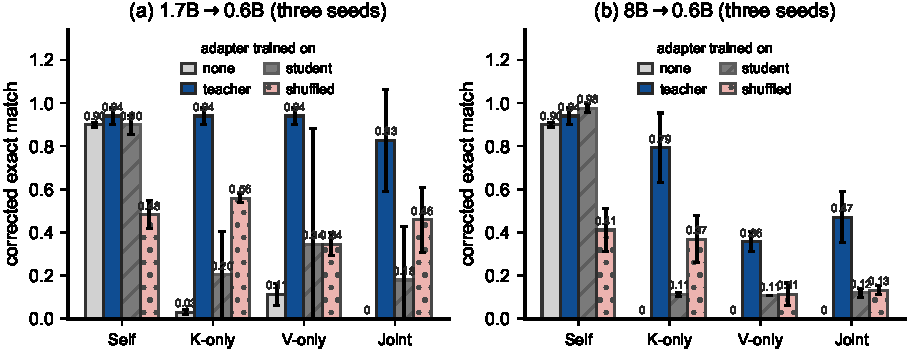
\includegraphics[width=\textwidth]{figures/fig_adapter.pdf}
\caption{消费适配器，留出测试集上的修正 EM（三个种子）。在标定教师 KV 上训练的
\texttt{o\_proj} 秩 8 修正恢复了教师臂；同一适配器若在学生 KV 上训练则不能，而在打乱文档
的教师 KV 上训练则居中。「none」组是未适配模型，其「Self」是它自身的缓存，适配器也会
改动该缓存，因此适配后的 Self 柱才是参照系。误差棒为报告了离散度时的种子间标准差。}
\label{fig:adapter}
\end{figure}

\subsection{留出的层选择}
\label{sec:layers-heldout}
在全部 $28$ 个学生层上做的验证扫描在每个种子上都选出 $(12, 16)$ 这一对，其中 $L_{12}$
在三个种子上都排第一，因此先前报告的值热点不是「在测试集上选择」造成的假象
（图~\ref{fig:layers}b）。在修正指标下，选中的这一对达到测试 EM $0.351$（各种子上
$0.339$、$0.357$、$0.357$），事后挑出的 $(8, 12)$ 对达到 $0.220$，注入全部层达到
$0.000$，而 Self 为 $0.899$。另一个为追求更高验证分而事后挑出的值对 $(12, 20)$ 只达到
$0.131$，在每个种子上都低于验证集选出的那一对：按验证集选择没有让我们付出代价，预注册
的选择反而是更强的那个。因此选择性注入值确实携带一些答案内容，但远远不足以构成任务迁移。

\begin{figure}[t]
\centering
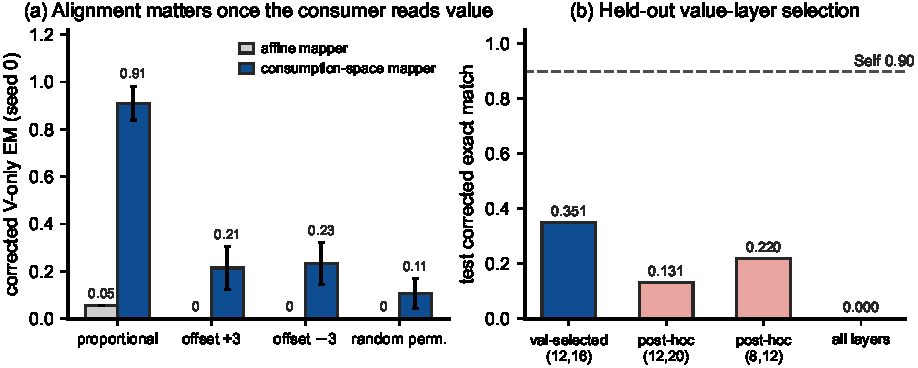
\includegraphics[width=\textwidth]{figures/fig_layers.pdf}
\caption{(a) 等深模型对 $1.7$B$\to0.6$B 上的层映射消融（种子 0），跑两次：一次用表示空间
中拟合的映射器（仿射），此时值臂被钉在地板上、层映射看起来无关紧要；一次用消费空间
映射器，此时按比例映射达到 $0.911$，而同样的打乱会代价掉其中大部分。在消费者能读取状态
之前，对齐是不可见的。(b) $8$B$\to0.6$B 上的留出值层选择（三个种子）：验证集选出的层对、
一个事后层对、以及全层注入，与 Self 参照对比。}
\label{fig:layers}
\end{figure}

% ============================================================================
\section{讨论}

\subsection{这一诊断确立了什么、没有确立什么}
\label{sec:discussion-scope}
这些证据支持四个陈述，我们让它们彼此分开，而不是把它们折叠成关于兼容性的单一主张。
\emph{(i) 评测。} Teacher-forced 似然并不能确立缓存的功能性复用：无内容的缓存（错误文档、
矩匹配随机、全零）复现了 K-only 似然增益的 $89$--$105\%$，却一道题也答不对；而我们在
早先所用实现中识别出的两个缺陷抬高了自家测量中的贪心 EM。第一点与任何实现细节无关；
第二点只覆盖我们审计过的代码。
\emph{(ii) 值迁移。} 在原始表示空间中对齐是不够的。仿射映射器把表示误差压到最小，却让
值臂不可用；而一个在学生消费值的位置上拟合的映射器能把它恢复（表~\ref{tab:mappers}）；
以文档为重采样单位时，被恢复臂的聚类 CI95 在种子 0 为 $[0.839, 0.982]$，仿射映射器为
$[0.018, 0.107]$，并且两个区间在三个种子上都不相交。表~\ref{tab:errorbudget} 的误差预算
把这一区别定量化，而表~\ref{tab:sweep} 的映射器目标扫描在 $198$ 个配置（而不是五个）上
确认了它：原始表示误差对仿射映射器最小，却在每一个 run 内都与 EM 正相关；而在学生的
注意力输出之后、以及经其 $o$ 投影之后测量的误差，在每一个 run 内都是强负相关，其
bootstrap 区间与原始误差区间不相交。五个变体的合并值为 $-0.10$、$-1.00$ 与 $-0.80$，
逐 run 范围分别是 $[-0.60,+0.05]$、$[-1.00,-0.80]$ 与 $[-1.00,-0.80]$；扫描以每个 run
$33$ 个配置得到同样的排序。
\emph{(iii) 键迁移。} 映射后的教师键会扰动接收方的路由（top-1 一致率 $0.59$--$0.70$，
而注意力余弦为 $0.93$--$0.97$），并且用学生注意力重新加权键拟合可以把该分歧压低
$17$--$43\%$ 却不移动任务臂（表~\ref{tab:routingkey}）。因此键侧失配是可诊断的，而据
这些证据，从路由侧缩小该分歧并不能修复任务臂；我们不主张逆命题，也无法断言路由兼容性是
必要条件，因为本文没有任何实验在「本来可以迁移」的条件下破坏路由兼容性。值臂从不接触
映射后的键，也不能用它解释。
\emph{(iv) 联合移交。} 完整移交必须同时满足两种兼容性，因此一贯地脆弱；它并不可靠地
把两个组件的收益合并起来。在四个模型对上，联合臂是三个教师臂中最低的，在剩下两个上等于
或高于单一臂，而在适配之后，它在旗舰对上落到 V-only 之下。

层对齐的作用取决于涉及哪一侧，而我们自己早先对它的解读是错的。在表示空间中，值臂停在
地板上，打乱层映射不付出任何代价，我们曾把这当成「对齐不重要」（第~\ref{sec:layer-align} 节）。
在消费空间中，映射器把值放在学生读取它的位置上，同样的打乱把 V-only EM 从 $0.911$ 压到
$0.11$--$0.23$。对齐是普通仿射映射器借自身地板所掩盖的一个前提条件，而不是消费方可以
忽略的量。

我们的证据并未确立「被恢复的信息就是教师的完整文档内容」。打乱文档的适配器对照居中，
而不是在地板上，因此该恢复有一部分是对类教师状态分布的适配，而不是针对具体文档。我们也
没有识别出让状态可读的机制。在键侧，我们能移动诊断量而不修复该臂：第~\ref{sec:two-failures} 节
的路由感知映射器把路由分歧压低 $17$--$43\%$，却仍让 K-only EM 停在地板上，且其打乱目标
对照并不更差。这只是一个针对单一干预的负结果，而不是「不存在任何键侧修复」的证明，它也是
我们的证据所能支持的最强陈述。

\subsection{意义}
\label{sec:implications}
如果跨模型缓存复用由消费者兼容性、而不是由线性映射是否存在的问题来决定，那么评测就应当
在修正评测器下报告任务指标并纳入无内容对照，而跨模型复用缓存的系统应当预留一小份消费侧
适配的预算。在我们的条件下，该适配约为 $0.7$M 参数，只在标定数据上训练，它在等深模型对
上恢复了 K、V 与联合臂的大部分、在旗舰对上恢复了其中一部分。由于该适配是在单一任务分布内
拟合并评测的，我们把这一要求表述为\emph{任务条件}功能兼容性：必须彼此兼容的是生产者、
消费者，以及状态被产生时所在的分布，三者合在一起。

\subsection{为什么一个负结果能与多个正面系统同时成立}
\label{sec:discussion-reconcile}
第~\ref{sec:rw-transfer}~节引用了报告近原生质量的跨模型缓存传输系统，而我们报告的是每个
教师臂都触底。两者可以同时为真，把这两种设置分开的三处差异是可检验的，而不是修辞。

\emph{映射器家族。}
本文的每一个映射器都是线性的：逐（层，头）岭回归、它的注意力质量重加权、两个消费空间目标，
以及它们之间的一参数插值。报告恢复的系统使用行为目标（例如对消费方自身预测的蒸馏）、
非线性分量，或可训练的修正阶段。因此我们的负结果限定的是线性映射器，而不是表示对齐本身。
“一个状态可以被线性映射重建、却仍然不可用”是我们的主张；它并不推出任何家族的映射器都无法
传输该状态。

\emph{键侧尚未在我们自己所主张的目标下检验。}
我们在消费方读取值的地方拟合值映射器，但对键只做了一次按学生注意力质量加权的表示空间回归。
这不是对称的实验。对称的做法是在消费方的 softmax 之前分数上回归——映射教师键，使
$Q_S\hat K^{\top}M^{\top}$ 接近 $Q_SK_S^{\top}$，这是同一参数上的闭式最小二乘问题——
我们把它未被执行记为本文的一个局限，而不是记为键侧不可修复的证据。


两种结果都会提供信息，而我们一种都还没有跑。如果对称目标仍让键臂停在地板上，那么「与接收方
softmax 之前的分数相匹配」就不是路由侧真正需要的东西，这一分解还隐藏着进一步的
query--key 交互。如果它恢复了键臂，交接的两侧就会对称地闭合：键走路由空间对齐，值走消费
空间对齐。
\emph{任务与指标。}
我们的主指标是在由隐知识图谱构造的问题上的精确匹配，测试文档数量很少；同期系统度量的是
长上下文、agent 与检索质量。精确匹配对“携带了大部分答案”的状态不作区分，而在我们的样本量下
它无法分辨部分恢复。因此我们把教师臂触底读作“精确匹配能接受什么”的陈述，并依赖
第~\ref{sec:controls}~节的内容对照与第~\ref{sec:two-failures}~节的路由诊断，
让论证独立于该指标成立。

这三处差异也说明了如果继续这项工作我们会先测什么：一个行为式的键目标、一个非线性映射器，
以及一个对部分恢复给予部分记分的指标。

\subsection{局限}
\label{sec:limitations}
\begin{itemize}
\item \textbf{范围。} 所有实验都在单一模型家族（Qwen3，$0.6$B--$8$B）与单一架构内进行，
  规模与头配置见第~\ref{sec:models} 节。我们不能声称跨家族或跨架构的普适性，也没有测试
  该家族之外的教师模型。
\item \textbf{任务分布。} 适配器在其被评测的同一任务分布上训练（问题与文档都是留出的，
  但语料与模板相同）。它度量的是消费的可修复性，而不是任务泛化；第二个域让这一点更锋利：
  即便把映射器与适配器\emph{在 SQuAD 内部}重新拟合，每个迁移臂在三个文档划分上仍只答对
  留出问题的 $0.000$（表~\ref{tab:squadrepair}）。我们在第~\ref{sec:adapter-results} 节
  区分了两种候选解释：同规模的、从合成域抽取的标定集以同样方式失败（每个迁移臂 $0.000$），
  而 $85$ 份混合两域的文档仍然失败（最好的臂 $0.067$，一道留出题），因此约束因素是分布
  而不是量。第二个域的留出 Self 只有 $0.20$--$0.40$，而且它只是一个域，所以我们把这读作
  「兼容性绑定在任务分布上」，而不是「任何映射器在那里都无法工作」的证明，并称之为
  \emph{任务条件性}。
\item \textbf{语料效应。} 每份文档都共享同一模板，且每份文档被大约七道题复用（测试集：
  $8$ 份文档产生 $56$ 道题）。因此错误文档对照作为内容对照是保守的，因为两份文档的主要
  差别只是它们提到的实体。四臂 EM 表报告种子间标准差、不给区间，但文档聚类的 EM 区间
  （每个种子八个簇）已由归档的逐样本行为三个种子全部算出，并在第~\ref{sec:teacher-states} 节
  引用。它们比逐样本区间更宽，并且确认而不是推翻排序——在 $8$B$\to4$B 上，V-only 为
  $0.43$--$0.45$，区间排除零，而 Self 为 $0.80$--$0.84$。种子间标准差仍然太窄、不足以
  倚赖，而聚类区间也仍然让该模型对的 V-only 臂远低于 Self。
\item \textbf{方差。} $1.7$B 适配器的联合臂在种子间从 $0.55$ 到 $0.96$，若干似然量也有
  很大的种子间波动（例如 $8$B$\to1.7$B 的 K-only 为 $+1.04 \pm 1.53$）。三个种子是小样本；
  对多数臂我们报告标准差而不是区间。
\item \textbf{映射器族。} 我们测试了线性与岭回归映射器，包括消费空间变体以及它们之间的
  单参数插值，但该族仍是线性的：非线性映射器未经测试，而它们可能改变「失败中有多少可归因
  于消费、而不是映射」这一比例。
\item \textbf{评测器来源。} 我们的修正数字来自自家评测器，它在三种学生规模的完整 $56$ 题
  Self 测试集上（图~\ref{fig:evalcheck}）、以及 $30$ 题的 SQuAD Self 集上都与全前缀参考
  实现做过校验。一致之处在抽取出的答案上（归一化 EM $0.929$--$0.982$）与首 token 分布上
  （top-1 一致率 $0.929$--$0.982$，中位 $KL$ $0.001$--$0.005$ nats），而不是逐 token 一致：
  贪心分词在 $7$--$21\%$ 的题目上分叉（取决于学生规模），单个最大 logit 误差为 $1.344$。
  我们对该残差做了归因而非任其不明——重复捕获、缓存往返与显式位置偏移都是精确的，全部差异
  都属于注意力内核路径，是 bf16 精度下的数值差异而不是实现缺陷。旧数字作为对照列在补充
  材料中，而不放在正文。
\item \textbf{未解释的基线差异。} Self EM 因学生而异（三个 $0.6$B 学生为 $0.899$、两个
  $1.7$B 学生为 $0.440$、$4$B 学生为 $0.815$）。原始与归一化精确匹配对每个学生都一致
  （原始的 $0.911$、$0.429$、$0.804$ 对归一化的 $0.911$、$0.429$、$0.804$；归一化下
  $0$ 道题从错翻转为对），失败计数为 $56$ 题中的 $5$、$32$、$11$。对归档的生成结果分类，
  $1.7$B 的每一次失败都是格式良好、但给出错误实体或数值的答案——同一模板中的另一个组件或
  工厂，或 yes/no 题上的相反极性——没有拒答、没有重复循环、没有空输出，也没有在解码上限处
  被截断的生成；$0.6$B 与 $4$B 的失败也是同类。因此 $1.7$B 的下凹是任务错误，而不是格式
  或抽取假象，但我们仍无法解释为什么该规模最弱。它不影响同一模型对内的臂间比较——我们的
  主张正是基于这种比较——但它意味着绝对 EM 水平不能跨模型对比较。
\item \textbf{部分种子覆盖。} 仍有两个结果只有种子 0：修复态下的层打乱
  （第~\ref{sec:layer-align} 节）与表~\ref{tab:ablation} 的投影消融。适配器因果性检验、
  映射器比较、第二个域以及两个对照套件都跑了三个种子，四臂扫描也全部如此。凡是对头条结论
  重要的比较，我们都用了三种子运行。
\item \textbf{旗舰对的因果性。} 在冻结最终 $20$ 轮适配器的条件下，破坏注入内容使正确臂
  与对照在 $1.7$B$\to0.6$B 上清楚地区分开（$0.905\pm0.083$ 对至多 $0.179$，边为
  $+0.68$ 到 $+0.86$，聚类区间排除零），但在 $8$B$\to0.6$B 上没有（$0.321\pm0.129$
  对 $0.107$--$0.286$，平均边 $+0.095$，两个聚类区间包含零）。我们无法排除旗舰对上的
  恢复有一部分是对类教师状态的通用适配。
\item \textbf{适配器训练方差。} 在固定种子下重复旗舰对适配器训练，正确因果臂在两次 run 中
  分别得到 $0.679$ 与 $0.429$。因此 $8$B 的边（$+0.095$）与适配器自身的训练方差相当，
  这是不该把旗舰对因果性视为已确立的第二个理由。我们报告三种子均值，但不把种子跨度当作
  置信陈述。
\item \textbf{已撤回的主张。} 本项目预注册的 G0 门限以及此前发表的所有 EM 数字均已撤回
  （第~\ref{sec:analyses} 节）。似然结果保留，但它们只是似然结果。
\end{itemize}

\subsection{未来工作}
\label{sec:future-work}
有三个方向：(i) 一种改变接收方路由、而不是重新加权拟合的键侧修复，因为
第~\ref{sec:two-failures} 节的路由感知映射器压低了路由分歧却不移动任务臂；(ii) 跨家族
评测（例如 Qwen$\to$Llama），以检验消费适配器的边界；(iii) 对映射器与适配器延迟相对重新
预填充的系统测量，它应当用实测成本替代附录~\ref{app:cost} 的参数计数启发式。

\subsection{结论}
\label{sec:conclusion}
跨模型 KV 传输是一个状态--消费者兼容性问题，我们的四臂设计让它的两侧保持分开。映射后的
教师键会扰动接收方的路由（键侧），而映射后的值在映射器被拟合到接收方消费它们的位置之前
一直不可用，无论其原始表示误差多小（值侧）。标准线性映射让教师状态变得可预测、并抬高
teacher-forced 似然，但在修正评测器下那些状态答不对问题，而无内容的缓存复现了让迁移看似
真实的似然增益。
本文的贡献不是「存在一个面向接收方的翻译器」——同期工作已经提供了它——而是这一分解、
对这条文献用来评测的代理量的审计、一个说明状态空间误差与消费空间误差\emph{符号}相反的
误差律，以及我们能够跨越和不能跨越的边界。
在消费者空间中拟合的映射器能在等深模型对上恢复值臂而不触碰任何消费方
权重——误差预算把该空间认定为靶子，因为原始表示误差无法按任务性能给映射器排序，而在
接收方读取状态处测量的误差可以——一个小的秩 8 输出投影适配则作为干预说明该侧的臂在那里
是可修复的。在旗舰对上，冻结的适配器能在等深对上读出注入内容，在旗舰对上却不行，其边停在
我们预注册的噪声带内；在第二个域上，即便把映射器与适配器都在该域内重新拟合，两者也都没
修复任何东西。一旦消费者能读取状态，层对齐就重新回到图景中，而这正是普通仿射映射器所
掩盖的。跨模型缓存复用的评测应当带内容对照地测量任务性能，而复用系统应当预期在适配被
拟合的任务分布内对消费者做适配。

% ============================================================================
\section{可复现性声明}
\begin{sloppypar}
数据生成、模型加载、修正评测器、对照套件、消费者空间映射器与消费适配器都实现在
\texttt{experiments/phaseB\_*.py} 中；重算文档聚类统计量、并对基线失败进行分类的分析
脚本位于 \texttt{scripts/}。图由 \texttt{paper/figures/gen\_paper\_figures.py} 生成，
该脚本记录了所转录的数值及其来源。修正四臂扫描、对照、对齐消融、留出层选择、映射器比较、
适配器运行与逐样本分解把 JSON 报告写入 \texttt{reports/}
（\texttt{phaseB\_fourarm\_seed*.json}、
\texttt{phaseB\_controls\_*.json}、
\texttt{phaseB\_mechanism\_*.json}、
\texttt{phaseB\_outaware\_*.json}、
\texttt{phaseB\_adapter\_*.json}、
\texttt{phaseB\_alignment\_repaired\_*.json}、
\texttt{phaseB\_evalcheck\_seed0.json}、
\texttt{phaseB\_selfdiag\_seed0.json}、
\texttt{phaseB\_squad\_seed*.json}、
\texttt{phaseB\_squad\_outaware\_seed0.json}、
\texttt{phaseB\_squad\_adapter\_seed0.json}，以及用于分解的
\texttt{factorial\_analysis.json}，
用于评测器归因的
\texttt{phaseB\_evalcheck\_residual\_seed0.json}、
\texttt{phaseB\_evalcheck\_attrib.json} 与
\texttt{phaseB\_evalcheck\_squad.json}，
用于冻结适配器因果性检验的 \texttt{phaseB\_adapter\_causal20\_*.json}，
用于预算的 \texttt{phaseB\_squadwithin\_split*.json}，
用于路由感知键映射器的 \texttt{phaseB\_routingkey\_*.json}，
用于映射器目标扫描的 \texttt{phaseB\_mappersweep\_*.json} 及其 \texttt{aggregate}，
以及用于量与分布对照的标定混合报告（\texttt{phaseB\_squadwithin\_*\_split*.json}），
还有用于文档聚类区间的 \texttt{cluster\_stats\_audit3.json}；
附录~\ref{app:cost} 中被替换掉的旧成本图归档在 \texttt{reports/archive/} 下。）
一份详细的更正说明（\texttt{paper/audit/METRIC\_CORRECTION.md}）记录了评测器缺陷、
它们产生的旧数字，以及每个修订后主张到其报告的对应关系。
\end{sloppypar}
\begin{thebibliography}{10}

\bibitem{bansal2021stitching}
Yamini Bansal, Preetum Nakkiran, and Boaz Barak.
\newblock Revisiting model stitching to compare neural representations.
\newblock In {\em Advances in Neural Information Processing Systems}, 2021.

\bibitem{chen2023accelerating}
Charlie Chen, Sebastian Borgeaud, Geoffrey Irving, et~al.
\newblock Accelerating large language model decoding with speculative sampling.
\newblock {\em arXiv preprint arXiv:2302.01318}, 2023.

\bibitem{dao2022flashattention}
Tri Dao, Dan Fu, Stefano Ermon, Atri Rudra, and Christopher R{\'e}.
\newblock Flashattention: Fast and memory-efficient exact attention with
  io-awareness.
\newblock {\em Advances in Neural Information Processing Systems}, 35, 2022.

\bibitem{dery2026latentalign}
Lucio~M. Dery, Zohar Yahav, Henry Prior, Qixuan Feng, Jiajun Shen, and Arthur
  Szlam.
\newblock Latent space communication via k-v cache alignment.
\newblock {\em arXiv preprint arXiv:2601.06123}, 2026.

\bibitem{dettmers2024qlora}
Tim Dettmers, Artidoro Pagnoni, Ari Holtzman, and Luke Zettlemoyer.
\newblock Qlora: Efficient finetuning of quantized language models.
\newblock {\em Advances in Neural Information Processing Systems}, 36, 2024.

\bibitem{frantar2023gptq}
Elias Frantar, Saleh Ashkboos, Torsten Hoefler, and Dan Alistarh.
\newblock Gptq: Accurate post-training quantization for generative pre-trained
  transformers.
\newblock {\em arXiv preprint arXiv:2210.17323}, 2023.

\bibitem{fu2026c2c}
Tianyu Fu, Zihan Min, Hanling Zhang, Jichao Yan, Guohao Dai, Wanli Ouyang, and
  Yu~Wang.
\newblock Cache-to-cache: Direct semantic communication between large language
  models.
\newblock In {\em International Conference on Learning Representations}, 2026.
\newblock arXiv:2510.03215.

\bibitem{heo2026crossmodel}
Taekyung Heo, Rasoul Shafipour, Ritchie Zhao, Maximilian Golub, Mohammad~Mahdi
  Kamani, Ritika Borkar, Makesh~Tarun Chandran, Pantea Zardoshti, and
  Bita~Darvish Rouhani.
\newblock Cross-model kv cache transfer in llm families: A closed-form linear
  mapping for prefill reuse.
\newblock {\em arXiv preprint arXiv:2608.03893}, 2026.

\bibitem{hinton2015distilling}
Geoffrey Hinton, Oriol Vinyals, and Jeff Dean.
\newblock Distilling the knowledge in a neural network.
\newblock {\em arXiv preprint arXiv:1503.02531}, 2015.

\bibitem{lee2026translators}
Jin-woo Lee, Minkyung Song, Junghyun Oh, Seunghoon Han, Gwangseon Jang, Soyoung
  Park, and Sungsu Lim.
\newblock Kv cache translation across heterogeneous large language models.
\newblock {\em arXiv preprint arXiv:2607.28979}, 2026.

\bibitem{leviathan2023fast}
Yan Leviathan, Matan Kalman, and Yossi Matias.
\newblock Fast inference from transformers via speculative decoding.
\newblock {\em International Conference on Machine Learning}, pages
  19274--19290, 2023.

\bibitem{su2024rope}
Jianlin Su, Murtadha Ahmed, Yu~Lu, Shengfeng Pan, Wen Bo, and Yunfeng Liu.
\newblock Roformer: Enhanced transformer with rotary position embedding.
\newblock {\em Neurocomputing}, 568:127063, 2024.

\bibitem{dare2024icml}
Le Yu, Bowen Yu, Haiyang Yu, Fei Huang, and Yongbin Li.
\newblock Language models are super mario: Absorbing abilities from homologous
  models as a free lunch.
\newblock {\em International Conference on Machine Learning}, 2024.
\newblock arXiv:2311.03099.

\bibitem{kivi2024icml}
Zirui Liu, Jiayi Yuan, Hongye Jin, Shaozhuo Zhai, Yuanzhi Chen, et~al.
\newblock Kivi: A tuning-free asymmetric 2bit quantization for kv cache.
\newblock {\em International Conference on Machine Learning}, 2024.
\newblock arXiv:2402.02750.

\bibitem{kvquant2024nips}
Coleman Hooper, Sehoon Kim, Hiva Mohammadzadeh, Michael~W. Mahoney,
  Kurt Keutzer, and Amir Gholami.
\newblock Kvquant: Towards 10 million context length llm inference with
  kv cache quantization.
\newblock {\em Advances in Neural Information Processing Systems}, 37, 2024.
\newblock arXiv:2401.18079.

\bibitem{ties2023merging}
Prateek Yadav, Derek Tam, Leshem Choshen, Colin Raffel, and Mohit Bansal.
\newblock Ties-merging: Resolving interference when merging models.
\newblock {\em Advances in Neural Information Processing Systems}, 36, 2023.
\newblock arXiv:2306.01708.

\bibitem{touvron2023llama}
Hugo Touvron, Thibaut Lavril, Gautier Izacard, et~al.
\newblock Llama: Open and efficient foundation language models.
\newblock {\em arXiv preprint arXiv:2302.13971}, 2023.

\bibitem{vaswani2017attention}
Ashish Vaswani, Noam Shazeer, Niki Parmar, et~al.
\newblock Attention is all you need.
\newblock {\em Advances in Neural Information Processing Systems}, 30, 2017.

\bibitem{cachebridge2026}
Xingyu Qu, Siyuan Lu, Zhiyu Chen, Sheng Wang, and Tao Lin.
\newblock Cachebridge: Efficient cross-model kv transfer for multi-model llm
  serving.
\newblock {\em arXiv preprint arXiv:2609.00891}, 2026.

\bibitem{acct2026}
Yuzhe Liu, Haolin Tian, and Tonghan Wang.
\newblock Acct: Asymmetric cross-llm context transfer.
\newblock {\em arXiv preprint arXiv:2610.42116}, 2026.

\bibitem{cachelink2026}
Haomiao Qiu, Yining Tang, Zijia Song, Ruizi Han, Ziyue Qiao, and Miao Zhang.
\newblock Cachelink: Functional kv transport for zero-prefill cross-model context
  handoff.
\newblock {\em arXiv preprint arXiv:2610.15509}, 2026.

\bibitem{kvlingo2026}
Val{\'e}rie Castin, Keitaro Sakamoto, Anastasiia Filippova, Jo{\~a}o Monteiro,
  Marco Cuturi, and Pierre Ablin.
\newblock Kv-lingo: Learning kv-cache translators with distillation.
\newblock {\em arXiv preprint arXiv:2609.32610}, 2026.

\bibitem{bridgekv2026}
Payman Behnam, Debopam Sanyal, Pranav Ponnusamy, Kusum Meda Ravi, Pranav Sastry,
  Mani Chandana Bandaru, Alind Khare, Myungjin Lee, and Alexey Tumanov.
\newblock Bridgekv: Large-model prefill and small-model decoding for llm inference
  via kv cache translation.
\newblock {\em arXiv preprint arXiv:2611.11761}, 2026.

\bibitem{contextreuse2026}
Yi Li, Dongming Jiang, Yi Zhao, and Bingzhe Li.
\newblock A universal context-reuse layer for cross-model kv sharing.
\newblock {\em arXiv preprint arXiv:2608.30963}, 2026.

\bibitem{heterofold2026}
Vincent-Daniel Yun, Woosang Lim, Haneul Yoo, Sungjoo Yoo, Murali Annavaram, and
  Sai Praneeth Karimireddy.
\newblock Prefill-free cross-family kv cache transfer for heterogeneous multi-agent
  llms.
\newblock {\em arXiv preprint arXiv:2609.32259}, 2026.

\bibitem{swarmtelepathy2026}
Abdulrahman Alabdulkareem, Irene Tenison, Yang Zhang, Yada Zhu, Boris Katz, and
  Dan Gutfreund.
\newblock Swarm telepathy: Prefill-free kv-cache transfer across families.
\newblock {\em arXiv preprint arXiv:2610.15095}, 2026.

\bibitem{rarecache2026}
Sreetama Sarkar, Saptarshi Mitra, Sitao Huang, Souvik Kundu, and Peter~A. Beerel.
\newblock Rarecache: Bridging the gap in cross-model kv cache reuse via rank
  disagreement-based selective recomputation.
\newblock {\em arXiv preprint arXiv:2610.11358}, 2026.

\bibitem{pactcheck2026}
Zhenyi Shen, Junru Lu, Wei Liu, Jiangnan Ye, Jiazheng Li, Di Yin, Xing Sun,
  Tameem Adel, Yali Du, Lin Gui, and Yulan He.
\newblock On the opportunities and challenges of prefill-to-autoregressive
  cross-model transfer.
\newblock {\em arXiv preprint arXiv:2611.06976}, 2026.

\bibitem{latentaudit2026}
Huixiang Zhang and Mahzabeen Emu.
\newblock Do latent channels actually communicate? a causal audit of latent
  multi-agent llm.
\newblock {\em arXiv preprint arXiv:2607.26773}, 2026.

\bibitem{funccache2026}
Zhikun Tao, Fangyong Jin, and Junping Zhao.
\newblock Can kv cache be reused across model updates? a deepseek-v4-flash case
  study.
\newblock {\em arXiv preprint arXiv:2611.14051}, 2026.

\bibitem{repairbudget2026}
Yuxing Peng, Zhiqing Tang, and Weijia Jia.
\newblock Where should a kv-cache repair budget go? distractor structure and
  contextual compatibility in non-prefix reuse.
\newblock {\em arXiv preprint arXiv:2611.06397}, 2026.

\bibitem{matcha2026}
Alina Sudakov, Guy Bar-Shalom, Fabrizio Frasca, and Haggai Maron.
\newblock Learning cross-model activation alignments with explicit many-to-many
  layer maps.
\newblock {\em arXiv preprint arXiv:2610.09058}, 2026.

\bibitem{prh2024}
Minyoung Huh, Brian Cheung, Tongzhou Wang, and Phillip Isola.
\newblock The platonic representation hypothesis.
\newblock In {\em International Conference on Machine Learning}, 2024.
\newblock arXiv:2405.07987.

\bibitem{structuregeo2026}
Junwon You, Mihyun Jang, Sangwoo Mo, and Jae-Hun Jung.
\newblock What converges in the platonic representation hypothesis? structure over
  geometry.
\newblock {\em arXiv preprint arXiv:2609.27252}, 2026.

\bibitem{relrepr2022}
Luca Moschella, Valentino Maiorca, Marco Fumero, Antonio Norelli, Francesco
  Locatello, and Emanuele Rodol{\`a}.
\newblock Relative representations enable zero-shot latent space communication.
\newblock In {\em International Conference on Learning Representations}, 2023.
\newblock arXiv:2209.15430.

\bibitem{qwen3report2025}
An Yang, Anfeng Li, Baosong Yang, et~al.
\newblock Qwen3 technical report.
\newblock {\em arXiv preprint arXiv:2505.09388}, 2025.
\end{thebibliography}

\appendix

\section{似然增量的分解}
\label{app:factorial}
本附录收录第~\ref{sec:layer-align} 节提到的探索性似然分解；它被移出正文，因为似然增益
本身并不是功能性迁移的证据（第~\ref{sec:controls} 节）。由于每个教师臂的修正 EM 都在
地板上，四臂设计只能在似然尺度上分解。表~\ref{tab:factorial} 报告 K 主效应
（K-only $-$ Self）、V 主效应（V-only $-$ Self）及其交互
（Joint $-$ K-only $-$ V-only $+$ Self），逐样本计算，并在与表~\ref{tab:main} 相同的 run 上
对种子取平均。

由此可得到若干模式，我们将其标注为探索性。V 主效应在四个模型对上为正、在两个上为负，
最大正值出现在 $8$B$\to1.7$B（$+5.63 \pm 0.04$），最大负值出现在 $4$B$\to0.6$B
（$-1.22 \pm 0.05$）。交互项在两个「大模型到小 $0.6$B」的模型对上为正
（$8$B$\to0.6$B 为 $+2.12 \pm 0.07$，$4$B$\to0.6$B 为 $+2.15 \pm 0.55$），在其余四个
模型对上为负（$-2.06 \pm 0.22$、$-2.67 \pm 0.09$、$-1.98 \pm 1.79$ 与 $-3.50 \pm 0.12$）。
因此它的符号随模型对变化；不存在一个适用于全部六个模型对的统一 K$\times$V 交互故事，
而且这些都是似然效应而不是任务效应。

对旗舰对，我们可以直接在逐样本差值上检验这一标题性不对称（$n=56$）：K 减 V 的配对差值
在种子 0 为 $+2.457$（CI95 $[+1.73, +3.29]$，$p=1.4\times10^{-9}$）、种子 1 为 $+2.720$
（$p=1.4\times10^{-10}$）、种子 2 为 $+3.361$（$p=7.5\times10^{-11}$）。在这个模型对上，
K 臂对似然的提升在每个种子上都以明显幅度超过 V 臂。这是关于似然的陈述；在修正 EM 上两个
臂都是 $0.000$。

\begin{table}[t]
\centering
\small
\caption{似然增量的分解（探索性），三个种子，$n=56$。K 主效应 $=$ K-only $-$ Self；
V 主效应 $=$ V-only $-$ Self；交互 $=$ Joint $-$ K-only $-$ V-only $+$ Self，基于逐样本
平均答案对数似然。K 与 V 两列等于表~\ref{tab:main} 中对应的 $\dll$ 列，此处重复列出以便
对照。}
\label{tab:factorial}
\begin{tabular}{lccc}
\toprule
模型对 & K 主效应 & V 主效应 & K$\times$V 交互 \\
\midrule
$8$B$\to0.6$B   & $+2.62{\pm}0.29$ & $-0.23{\pm}0.19$ & $+2.12{\pm}0.07$ \\
$4$B$\to1.7$B   & $+2.90{\pm}0.09$ & $+2.91{\pm}0.21$ & $-3.50{\pm}0.12$ \\
$4$B$\to0.6$B   & $+1.58{\pm}0.02$ & $-1.22{\pm}0.05$ & $+2.15{\pm}0.55$ \\
$8$B$\to1.7$B   & $+1.04{\pm}1.53$ & $+5.63{\pm}0.04$ & $-1.98{\pm}1.79$ \\
$1.7$B$\to0.6$B & $-0.82{\pm}0.02$ & $+0.63{\pm}0.17$ & $-2.06{\pm}0.22$ \\
$8$B$\to4$B     & $+8.52{\pm}0.28$ & $+2.52{\pm}0.07$ & $-2.67{\pm}0.09$ \\
\bottomrule
\end{tabular}
\end{table}

\section{用映射器替代缓存传输的成本启发式}
\label{app:cost}
为完整起见：用本文实际使用的映射器——每（层，头）一个仿射映射，每侧
$L_S\cdot H\cdot(D^2+D)$ 个参数，两侧都以 fp32 存储——$28$ 层学生的参数数为 $7.40$M
（$28.2$ MiB），而 fp16 KV 为每 token $112$ KiB，字节交叉点约在 $260$ token。这个数字
是一个启发式：它统计的是映射器参数而不是传输时间，忽略了量化与缓存，也不影响上面
关于状态--消费者的结论。本文早先版本引用了大得多的交叉点，因为它按每层一个
$1024\times1024$ 映射来计，而不是按第~\ref{sec:mappers} 节定义的每（层，头）映射。

\end{document}
